% !Mode:: "TeX:UTF-8"
\documentclass[final,MD,numbers,times]{cumtthesis}
\usepackage{fontspec}
\setmainfont{Times New Roman}
\usepackage{listings}
\usepackage{multirow}
\usepackage{indentfirst}
\usepackage{tikz}
\usepackage{etoolbox}
\usepackage{color}
\usepackage{algorithm}
\usepackage{algorithmic}
\usepackage{float}
\usepackage{rotating}
\usepackage{gensymb}
\usepackage{enumerate}
\usepackage[a4paper,left=3.17cm,right=3.17cm,top=2.54cm,bottom=2.54cm]{geometry}
\usetikzlibrary{matrix,calc,shapes,backgrounds,patterns,positioning,decorations.pathreplacing}
%=================================== 数学符号 =================================%
\newcommand{\rtn}{\mathrm{\mathbf{R}}}
\newcommand{\N}{\mathrm{\mathbf{N}}}
\newcommand{\AS}{~\mathrm{a.s.}}
\newcommand*{\PR}{\mathrm{\mathbf{P}}}
\newcommand*{\EX}{\mathrm{\mathbf{E}}}
\newcommand*{\dif}{\,\mathrm{d}}
\newcommand*{\F}{\mathcal{F}}
\newcommand*{\prs}{\dif\PR-\mathrm{a.s.}}
\newcommand*{\pts}{\dif\PR\times\dif t-\mathrm{a.e.}}
\newcommand{\Ito}{It\^{o}}
\newcommand{\tT}[1][0]{[#1,T]}
\newcommand{\intT}[2][T]{\int^{#1}_{#2}}
\newcommand{\s}{\mathcal{S}}
\newcommand{\me}{\mathrm{e}}
\newcommand{\one}[1]{{\bf 1}_{#1}}
\newcommand{\Mm}{{\rm M}}
\newcommand{\circled}[2][]{\tikz[baseline=(char.base)]
    {\node[shape = circle, draw, inner sep = 1pt]
    (char) {\phantom{\ifblank{#1}{#2}{#1}}};%
    \node at (char.center) {\makebox[0pt][c]{#2}};}}
\robustify{\circled}
\setlength{\intextsep}{10.0pt plus 2.0pt minus 2.0pt}


\floatname{algorithm}{算法}
%\newcommand\forthsection[1]{\noindent \S #1}
\renewcommand{\algorithmicrequire}{ \textbf{输入:}} %Use Input in the format of Algorithm  
\renewcommand{\algorithmicensure}{ \textbf{输出:}} %UseOutput in the format of Algorithm
\renewcommand\theequation{\arabic{chapter}-\arabic{equation}}
\renewcommand{\thealgorithm}{\arabic{chapter}-\arabic{algorithm}}
% \let\oldcite=\cite
% \renewcommand\cite[1]{
%   \textsuperscript{\oldcite{#1}}
% }
\DeclareMathOperator*{\sgn}{sgn}
%=================================== 数学符号 =================================%
%=================================== Code Style ==============================%
\definecolor{mygreen}{rgb}{0,0.6,0}
\definecolor{mygray}{rgb}{0.5,0.5,0.5}
\definecolor{mymauve}{rgb}{0.58,0,0.82}
\lstset{
  aboveskip=3mm,
  belowskip=3mm,
  showstringspaces=false,
  columns=flexible,
  basicstyle={\normalsize\ttfamily},
  numbers=left,
  frame=L,
  numberstyle=\tiny\color{mygray},
  keywordstyle=\color{blue},
  commentstyle=\color{mygreen},
  stringstyle=\color{mymauve},
  breaklines=true,
  breakatwhitespace=true,
  tabsize=3,
  framextopmargin=2pt,framexbottommargin=2pt,abovecaptionskip=-3pt,belowcaptionskip=3pt,  
  xleftmargin=1em, % 设定listing左右的空白
}
%=================================== Code Style ==============================%
%\CTEXsetup[indent={0pt}]{section}
\begin{document}
\frontmatter

%--------输入中文论文题目
\CLunWenTiMu{基于Spatial-Spark海量网络空间数据分析与应用}

%--------输入英文论文题目
\ELunWenTiMu[0.95]{Analysis and Application about Internet Spatial Data Based on Spatial-Spark}

%--------输入论文作者
\ZuoZhe{高峰}

%--------输入导师职称,导师姓名
\DaoShi[教授]{高井祥}
\DiErDaoShi[副教授]{孙久运}

%--------输入毕业时间
\BiYeShiJian{2017}{6}

%--------输入中图分类号
\ZhongTuFenLeiHao{P2}

%--------输入UDC
\UDC{910.1}

%--------输入密级
\MiJi{公开}

%--------输入毕业学校, 默认是中国矿业大学
%\BiYeXueXiao{}

%--------输入学校代码, 默认是10290
%\XueXiaoDaiMa{}

%--------输入学位类别
\XueWeiLeiBie{工学}

%--------输入培养单位
\PeiYangDanWei{环境与测绘学院}

%--------输入学科专业
\XueKeZhuanYe{大地测量学与测量工程}
%--------输入研究方向
\YanJiuFangXiang{3S技术集成及其应用}

%--------输入答辩委员会主席
\DaBianWeiYuanHuiZhuXi{吴侃}

%--------输入评阅人
\PingYueRen{}

%--------制作封面命令
\makecover

%--------致谢
\begin{acknowledgements}
矿大七年的求学经历即将结束,纵有千万般不舍,也要走向社会,用自己的在矿大学到的知识回报这个社会。作为矿大
新百年的学子,矿大「好学力行、求是创新、艰苦奋斗、自强不息」的校训将成为我人生中的座右铭,在接下来
的人生中,矿大精神将永远激励我前进,在这再次感谢矿大对我培养。

首先感谢我的导师高井祥老师和孙久运老师,您们是我研究生生涯中的指明灯,指引我走向学术生涯道路。两位老师孜孜不倦的精神使
我受益终身,你们为我提供了优越的科研环境,耐心和用心地指导我们开展学术活动,严谨的科研思维
和扎实的工作作风是我的楷模。当我申请去中科院电子所苏州研究院实习,你们坚定的支持是我最大的动力,再次感谢你们。

还要感谢中科院电子所苏州研究院胡岩峰院长,张昱老师、廉海明老师,在苏州实习期间,是你们的指导使我扩展了科研的视野。
将我储备的专业知识在实践中加以应用,也让我认识到自己专业领域的不足。在苏州也认识了一些有趣的人,这些为我
的人生增加了许多美好的回忆,谢谢你们能提供给我实习的机会。

感谢实验室张明杰、杨文环师兄和许世娇、王慧师姐,是你们在学习和生活上给了我巨大的帮助,你们的帮助使我快速地适应
了研究生生活。感谢实验室同门张新耐、赵冰峰、孙梦娇和李光雨,非常有幸和你们一起学习生活,一起成长,非常感谢你们
在我外出实习期间帮我处理学校一些事务,和你们在一起的日子是我人生中一段宝贵的财富。

感谢论文中所有参考文献的作者,是你们杰出的工作,让我产生一点点灵感,你们是巨人的肩膀。还要感谢\LaTeX
中文社区的肖立顺师兄,你无偿提供的矿大毕业论文\LaTeX{}模板,使我能够使用优美的\LaTeX{}完成论文排版工作。

也要感谢远在家乡的家人,是你们坚定不移的支持,是我读研的全部动力,这份理解和付出无法报答,希望你们身体健康,永远
幸福。

最后,感谢各位专家和老师,在百忙之中评阅本论文并提出宝贵的意见和建议,我会聆听你们的教导继续努力。
\end{acknowledgements}

%--------中文摘要
\begin{cabstract}
% 信息是当代社会重要的决策资源,随着移动互联网的迅速发展,以新浪微博为代表的
% 社交空间数据呈现爆炸式增长,然而这些数据存在异构性、不规则性和海量性等
% 特点,使得空间数据分析、空间数据挖掘和信息提取愈发难以处理。
% 随着移动互联网的迅速发展,以新浪微博为代表的社交网络数据呈现爆炸式增长,其中
% 包含的空间数据更值得关注和研究。然而这些数据存在着异质性、不规则性和海量性等
% 特点,使得空间数据查询、空间数据挖掘和空间知识提取愈发难以处理。

数字城市是智慧城市重要的组成部分,也同时面临着海量空间数据获取、管理、分析和挖掘等挑战。
移动互联网的发展使得网络空间数据呈现爆炸式增长,其中蕴含的信息对智慧城市建设有着重要的
参考建议,然而这些数据存在着异质性、不规则性和海量性等特点,使得空间数据查询、空间数据挖掘和
空间知识提取愈发难以处理。

传统的空间分析工具面对上述需求往往捉襟见肘,本文对当前流行的并行计算框架Spark进行空间扩展,
构建Spatial-Spark并行空间计算框架。以此为基础,对海量新浪微博POI进行同位模式
挖掘,对全国新浪微博用户空间位置进行人口网络图分析,本文所作的工作和结论如下:

(1)对Spark RDD((Resilient Distributed Datasets)进行空间维度上扩展,对点、线和面构建了相应的Spatial RDD,
支持海量空间数据读写、空间坐标转换和分区空间数据索引。提供空间拓扑查询、空间K邻居查询和空间连接查询三个常用的
空间查询模块,通过搭建Hadoop/Spark计算集群,验证了Spatial-Spark在处理海量空间数据方面的优势。

(2)使用新浪微博API获取全国范围内微博POI数据,对其进行同位模式挖掘。首先分析同位模式
挖掘算法的关键,使用Spatial-Spark对全连接算法进行并行化设计。对上海、武汉和重庆三市二阶模式
进行比较,不同城市呈现不同模式;选择距离阈值$d=500\text{\textrm{m}}$和空间参与度阈值$0.6$,
对北京市微博POI类别进行同位模式挖掘,结果显示阶数越高越呈现商业聚集模式,
其中最高六阶模式为(KTV,中餐厅,咖啡厅,甜品店,美容美发店,酒吧)。

(3)根据全国新浪微博用户在$2016$年春节期间的空间位置数据,使用Spatial-Spark构建全国城市之间人口流动网络图。
首先计算每个城市人口流入量、流出量和流入流出比,发现全国城市在春节期间人口流动呈现多样性;然后采用PageRank算法
计算城市在人口流动网络图中的权重,发现城市权重与城市GDP发展的存在相关性,并根据权重将中心城市划分四个层次;
最后对社群挖掘算法进行并行化改进,对人口流动网络图进行社群挖掘,发现城市联系紧密性与省份有关,地理位置对其
影响很大,但也存在突破地理空间位置限制的城市。

本文包含图\ref{totalfigure}幅,表\ref{totaltable}张,参考文献\ref{totalbib}篇。
%--------中文关键词
\CKeyWords{Spatial-Spark, 新浪微博, 同位模式, 网络分析}
\end{cabstract}

%--------英文摘要
\begin{eabstract}
% Information plays a signifcant role for strategy making in moderen society. As the tremendous 
% increment of internet, the social spatial data implying folk's behavior has been explosing. 
% Howerver, the heterogeneous, irregular and countless data causes the spatial data's analysis,
% mining and knowledge discovering becoming more difficult to handle.
% As the tremendous development of mobile internet, the social networks, represented by Weibo, are 
% releasing explosing amount of data. The spatial data in that is deserved of particular attention and 
% reserarch. Howerver, the heterogeneous, irregular and countless data leads the spatial data's analysis,
% mining and knowledge discovering becoming more intractable.
Digit City plays a vital role in smart city, and facing explosing amount data fetch, management, analysis
and mining challenges. Mobing internet developments cause the cyber spatial data increaing unbelievablely which
contains much informations for building the smart cities. Howerver, the heterogeneous, irregular and countless data leads the spatial data's analysis,
mining and knowledge discovering becoming more intractable.

Traditional spatial analysis method cannot meet the above requires, so this thesis builds the parallel 
spatial computing framwork, called Spatail-Spark, based on popular open-source parallel computing framwork.
Using this framework, it mines the spatial co-location pattern in Weibo's POIs and population graph according to 
the Weibo users's spatial locations. The achievements and conclusions of this thesis are listed as follows:

(1) It expands the Spark RDD in spatial geometries called Spatial RDD, including point, line and polygon. 
And those RDDs support the spaital data reading and writing, spatial coordinates converting and spatial 
index building in separate partition. It also provides three spatial query modules: sptaial topology query,
spatial K near neighbour query and spatial join query. At last, it designs experiments to figure out the 
efficiency of Spatial-Spark by various comparsions.

(2) After fetching out Weibo's POIs through Weibo's API, it conducts the spatial co-location pattern mining
algorithm in those data. It analysis the vital key of spatial co-location pattern and redesigns the parallel 
% algorithm for efficient perform using Sptial-Spark. It comes out that the patterns shows more commercial 
% characteristics when the pattern's order is bigger on the condition that 
% the spaital distance threshold is $500$ meters and the participating index threshold is $0.6$. Moreover, the 
% six order pattern is (KTV, Chinese Restaurant, Coffe Bar, Dessert Stall, Barber Shop, Bar Pub).
algorithm for efficient performance using Spatial-Spark. It comes out that the there are huge differences 
among the different cities, taking the Shanghai, Wuhan and Chongqing. It also provides that the patterns shows more commercial 
characteristics when the pattern's order is bigger on the condition that 
the spaital distance threshold is $500$ meters and the participating index threshold is $0.6$. Moreover, the 
six order pattern is (KTV, Chinese Restaurant, Coffe Bar, Dessert Stall, Barber Shop, Bar Pub).

(3) It constructs the cities floating population graph using Spatial-Spark from the national Weibo's users 
location in 2016 Chinese New Year holiday. At first, it calculates the popluation amount of flow-in and flow-out,
and flow ratio, which displays the diversity of floating population among the national cities. Then it figures
out the national cities' weights in floating population network under PageRank algorithm. It finds out the relationship
between city's weight and city's development and divides the natianal cities into four levels. Lastly, it applys the 
parallel community mining algorithm in this network and uncovers the phenomenon that the cities's popluaiton relationships are 
almost limited by the provinces and there are also some exceptional cases. 

This thesis contains \ref{totalfigure} figures, \ref{totaltable} tables and \ref{totalbib} references。
%--------英文关键词
\EKeyWords{Spatial-Spark, Weibo, Co-Location Pattern, Graph Analysis}
\end{eabstract}

%--------插入中文目录
\tableofcontents
%--------插入英文目录
\tableofecontents

%--------插入图清单
\listoffigures
%--------插入表清单
\listoftables
%--------变量注释表

\begin{notation}[2.5cm]
\item[$min\_s$] 最小支持度
\item[$min\_c$] 最小置信度
\item[$R$] 空间邻近关系
\item[$row\_instance$]  行实例
\item[$table\_instance$] 表实例
\item[$PR(c,f_i)$] 空间参与率
\item[$PI(c)$] 空间参与度
\item[$min\_prev$] 最小参与度
\item[$\delta_i$] 流入量
\item[$\omega_i$] 流出量
\item[$\psi_i$] 流入流出比
\item[$Q$] 模块值
\item[$\Delta Q$] 模块增益值
\end{notation}

%================================== 正文开始 ==================================%
\mainmatter

\section{绪论}

\begin{frame}{绪论}
    \begin{columns}
        \begin{column}{0.5\textwidth}
        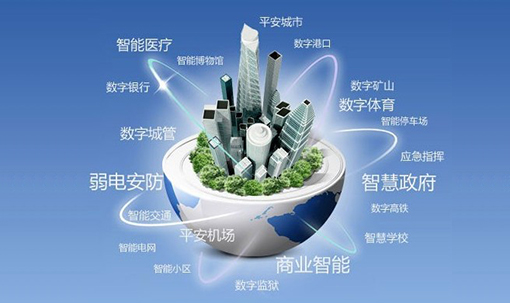
\includegraphics[scale=0.3]{figures/smartcity.jpg}
        \end{column}

        \begin{column}{0.5\textwidth}
        \textbf{智慧城市:} 
        
        数字城市、物联网、云计算
        \vspace{2em}

        \pause
        \alert{数字城市}
        \begin{itemize}
        \item 空间信息快速获取技术
        \item 海量空间数据管理技术
        \item 空间信息可视化技术
        \item 空间数据分析挖掘技术
        \item $\ldots$
        \end{itemize}
        \end{column}
   \end{columns}
\end{frame}

\begin{frame}{绪论}
    \textbf{移动互联网发展}

    \alert{LBS应用}
    打车软件、O2O软件、社交网络软件

    \vspace{2em}
    \pause
    \textbf{意义}
    \begin{itemize}
        \pause
        \item 对个人而言(智慧生活)
        \pause
        \item 对商业公司而言(智慧商业)
        \pause
        \item 对政府决策部门而言(智慧政府)
    \end{itemize}
\end{frame}

\begin{frame}[t]{绪论}
% \alert{海量数据处理}

% 业界使用Hadoop并行计算框架,但是存在处理速度慢、计算抽象层次较低等缺陷。

% \pause
% Spark是新型的并行计算框架,内存计算速度快,算子表现力丰富。但是对空间数据类型和空间数据操作支持不够。

\begin{columns}
    \begin{column}{0.4 \textwidth}

        \begin{center}
        \alert{海量数据处理}

        \vspace{1em}
        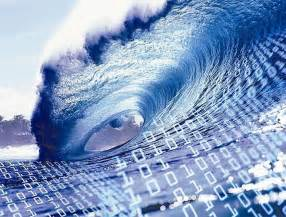
\includegraphics[height=3.5cm]{figures/seaamountdata.jpeg}
        \end{center}


    \end{column}

    \pause
    \begin{column}{0.6 \textwidth}

        \begin{center}
            \alert{并行计算}

            \vspace{1em}
            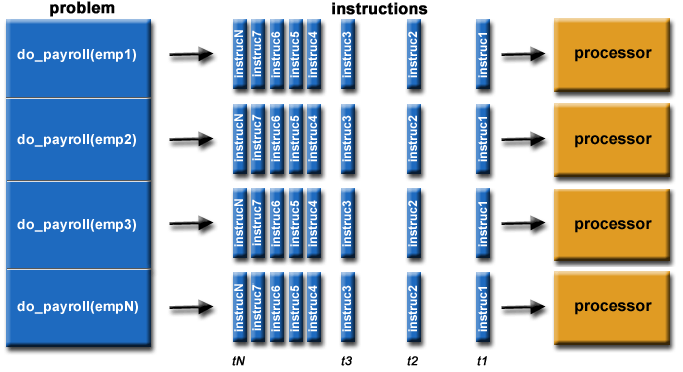
\includegraphics[height=3.5cm]{figures/parallelcomputation.png}
        \end{center}
       
    \end{column}

\end{columns}

% \vspace{2em}

% \pause
% \alert{并行化算法设计}

% 空间数据挖掘算法并没有针对并行化计算框架进行设计。

\end{frame}

\begin{frame}[c]{绪论}
    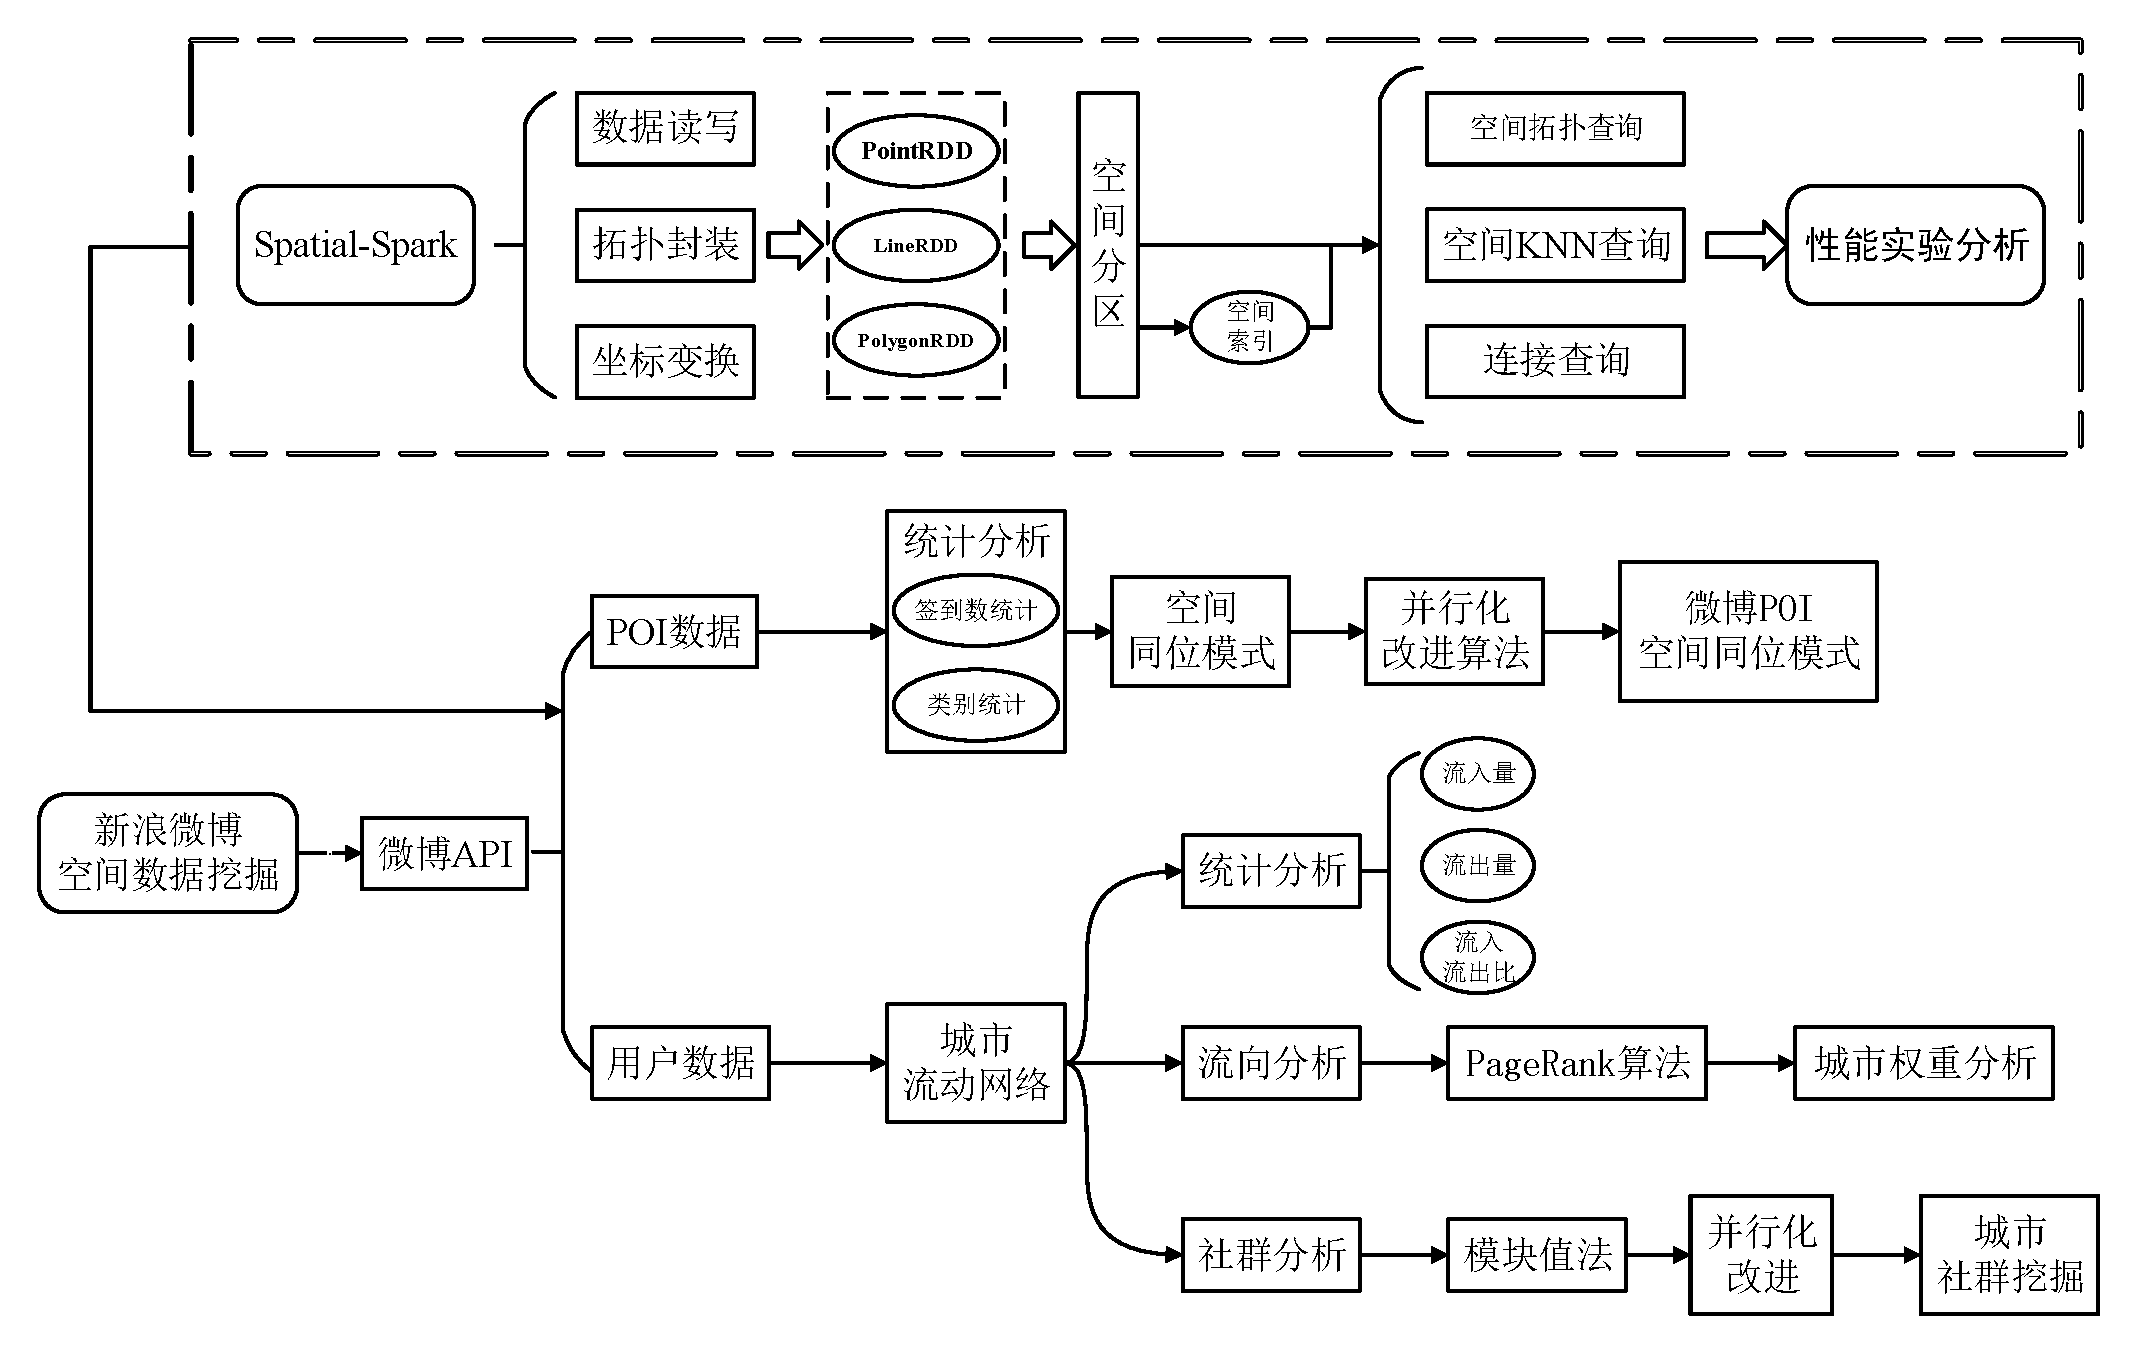
\includegraphics[scale=0.3]{figures/technology_route.pdf}
\end{frame}
\section{相关技术}

\subsection{Hadoop}

\begin{frame}[t]{相关技术(Hadoop)}
    \textbf{Hadoop}是Apache基金会推出的大数据计算平台
    
    \pause
    HDFS(Hadoop Distributed File System)

    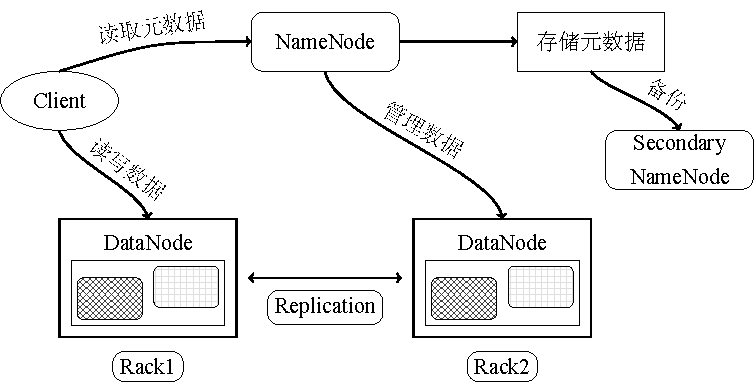
\includegraphics[scale=0.8]{figures/hdfs.pdf}
\end{frame}

\begin{frame}[t]{相关技术(Hadoop)}
    \textbf{Hadoop MapReduce}

    \pause
    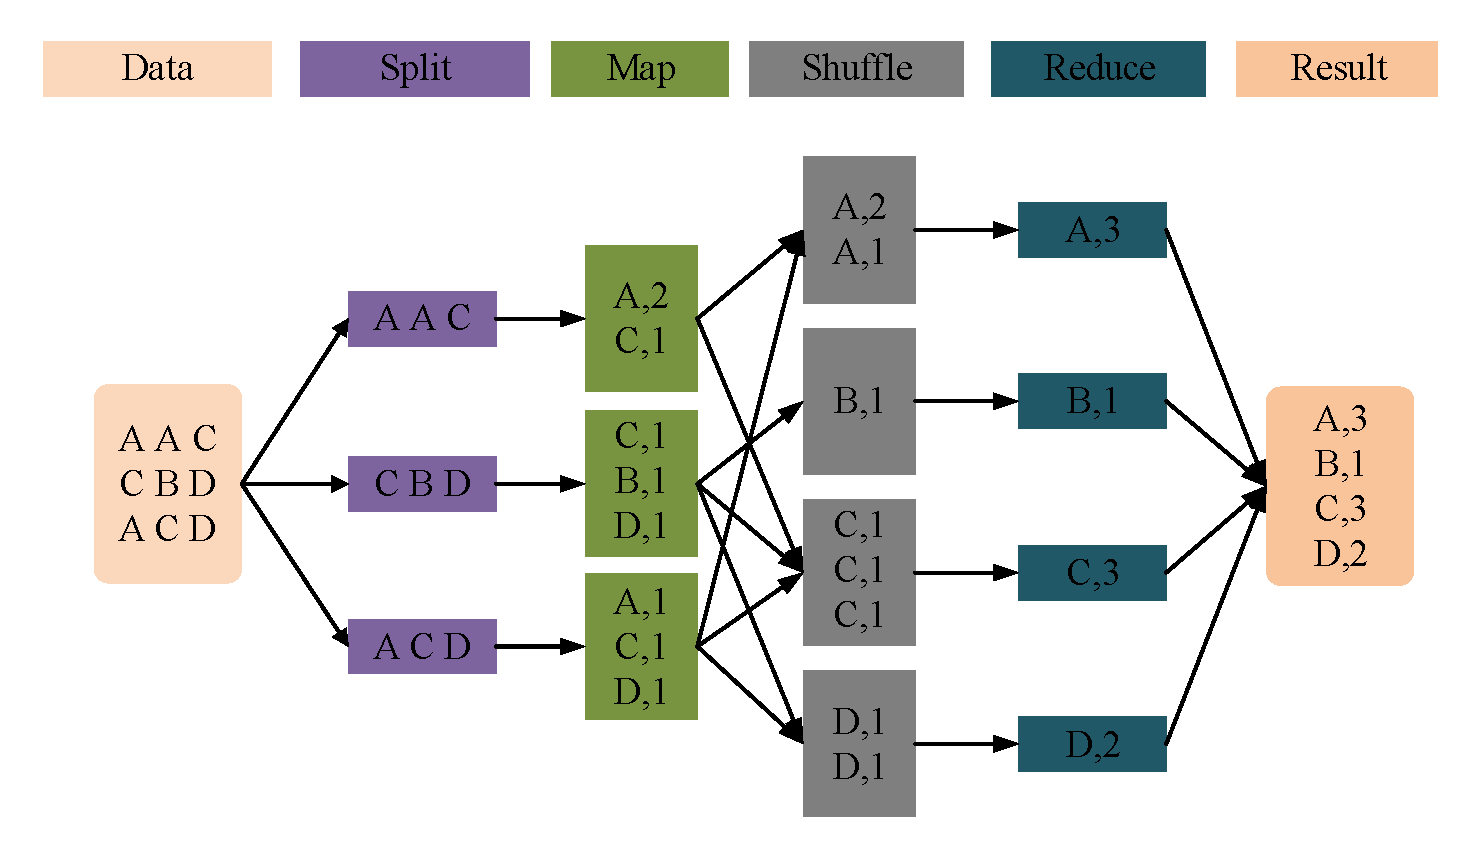
\includegraphics[scale=0.4]{figures/mapreduce.pdf}

    \pause
    \vspace{-1em}
    \begin{center}
    \alert{缺陷: }单点故障、算子抽象、IO操作频繁
    \end{center} 
\end{frame}

\subsection{Spark}

\begin{frame}[c]{相关技术(Spark)}
    \begin{columns}
        % one column
        \begin{column}{0.5 \textwidth}
            \textbf{Spark}技术生态系统

            \vspace{0.5em}
            \begin{figure}
                \centering
                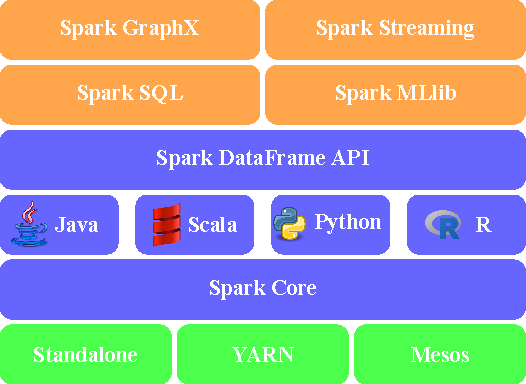
\includegraphics[scale=0.6]{figures/spark.pdf}
            \end{figure}            
        \end{column}

        %next column
        
        \pause
        \begin{column}{0.5 \textwidth}
            \begin{itemize}
                \item \textbf{Spark SQL}: 类SQL语言查询结构化数据
                \item \textbf{Spark MLlib}: 常用机器学习算法Spark实现
                \item \textbf{Spark GraphX}: 分布式图及其计算Spark实现
                \item \textbf{Spark Streaming}: Spark流应用计算框架
            \end{itemize}
        \end{column}
    \end{columns}
\end{frame}

\begin{frame}[t]{相关技术(Spark)}
    弹性分布式数据集(RDD)是Spark的核心抽象,在内存中已被分区、只读的、并提供
    一组丰富的操作方式的数据\textbf{集合}

    \vspace{2em}
    \pause
    \alert{RDD算子}
    \begin{itemize}
        \item \textbf{Transformation} 
        \item \textbf{Action}
    \end{itemize}

\end{frame}

\begin{frame}[c]{相关技术(Spark)}
    \begin{columns}
        \begin{column}{0.5 \textwidth}
            Spark一栈式解决方案的\alert{优势:}
            
            \vspace{0.5em}
            \begin{itemize}
                \item 快速处理,内存计算
                \item 通用性,技术方案无缝集成
                \item 与Hadoop集群集成
            \end{itemize}
        \end{column}

        \pause
        \begin{column}{0.5 \textwidth}
            Spark在处理海量空间数据\alert{劣势:}

            \vspace{0.5em}
            \begin{itemize}
                \item 不支持空间数据类型
                \item 不支持空间操作
                \item 没有空间数据优化
            \end{itemize}
        \end{column}
    \end{columns}

\end{frame}

% \subsection{微博数据接口}

% \begin{frame}[c]{微博数据接口}
%     新浪微博提供了API方便第三方程序访问微博丰富的数据资源

%     \begin{figure}
%         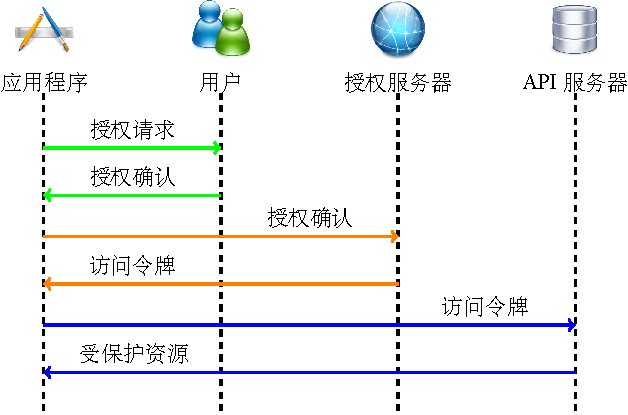
\includegraphics[scale=0.8]{figures/api.pdf}
%     \end{figure}
% \end{frame}

% \begin{frame}[t]{微博数据接口}
%     \alert{HTTP Get}请求

%     \vspace{0.5em}
%     \pause
%     \begin{itemize}
%     \item location/geo/address\_to\_geo $\rightarrow$  根据地址返回地理信息坐标 
%     \item location/pois/show\_batch $\rightarrow$ 批量获取POI点的信息
%     \item location/citycode $\rightarrow$ 城市代码对应表
%     \item place/nearby/pois $\rightarrow$ 获取附近的POI点
%     \end{itemize}
% \end{frame}


\chapter{Spatial-Spark计算框架}{Spatial-Spark Computation Framework}
\section{空间数据分析处理}{Procession of Spatial Data}
\subsection{空间数据格式}
空间数据量大且空间数据格式也是各式各样。开放地理空间信息联盟(Open GIS 
Consortium, OGC)定义了一些空间矢量数据格式\cite{Bychowski2003Open},方便能够进行空间数据分析
处理和交换,下面介绍几种常用的空间矢量数据格式。

(1)WKT数据格式

WKT(Well-Know-Text)数据格式以文本形式描述,用来表示点,线和面空间对象,见表\ref{tab:wktdata}。
\begin{table}
    \centering
    \caption{WKT矢量空间数据}{Vector spatial data in WKT}
    \label{tab:wktdata}
    \tabulinesep=1.5mm
    \begin{tabu}to 0.8\linewidth{X[1.1,c]X[2.5,c]}
        \tabucline[0.10em]-
        \rowfont[c]{} 几何类型 & WKT表示方式 \\
        \tabucline-
        ST\_Point & POINT(10.05 10.28) \\
        ST\_LineString & LINESTRING (10.05 10.28 , 20.95 20.89) \\
        ST\_Polygon & POLYGON((10 10, 10 20, 20 20, 20 15, 10 10)) \\
        \tabucline[0.10em]-
    \end{tabu}
\end{table}

(2)GeoJSON数据格式

GeoJSON数据是通过JSON数据表达简单的数据格式,如点、线、多边形和这些几何类型的集合以及他们非空间属性信息,表达方式如下:
\begin{lstlisting}[
  morekeywords={type,geometry,coordinate,fields}
]
{
  "type":"feature",
    "geometry":{
      "type":"LineString",
        "coordinate":[[[-100.50,57.14],[-89.45,62.17],[-37.21,79.73]]],
        "fields":{
            "prop1":"value","prop2":"string"
            }                
    }
}
\end{lstlisting}

由于JSON格式在序列化和网络传输中的优势,非常适合分布式的数据存储,空间数据和属性数据都存储在普通的文本中。

(3)GML数据格式  

GML(Geography Markup Language)是以XML格式的空间数据表达形式,并使用XML Schema文件
定义技术,目前版本为$2.1.1$。XML Schema具有类型继承、命名空间等特性,通过XLink来表现地理空间实体的关系。
\begin{lstlisting}[language=XML]
<PhotoCollection xmlns="http://www.myhotos.org"
    xmlns:gml="http://www.opengis.net/gml"
    xmlns:xsi="http://www.w3.org/2001/XMLSchema-instance"
    xsi:schemaLocation="http://www.myphotos.org" >
    <items>
      <item>
        <name>Lynn</name>
          <description>A shot of the falls</description>
          <where>North Vancouver</where>
          <position>
            <gml:Point srsDimension="2" 
              srsName="http://www.opengis.net/def/crs/EPSG/0/4326" >
                <gml:pos>49.40 -123.26</gml:pos>
            </gml:Point>
          </position>
      </item>
    </items>
</PhotoCollection>
\end{lstlisting}

\subsection{空间数据转换}
空间数据来源各异,每种数据来源有各自的坐标参考系统,如GPS接收机获取的地理空间数据
是以WGS$84$坐标系统为基准;摄影测量往往采用该区域最适宜的坐标参考系统为基准。不同的
大地坐标系统和平面投影系统往往使得空间数据处理和分析正确性得不到保证,因此很有必要
将多源空间数据纳入到同一个空间参考系统下。

Proj.$4$是开源GIS中著名的地图投影库\cite{Urbanek2012proj4},在GRASS GIS, MapServer, PostGIS等众多GIS
软件中都直接或者间接使用Proj.$4$,$2008$年OSGeo将Proj.$4$纳入到MetaCRS的一部分,Proj.$4$
的主要功能是提供了大地坐标系和投影坐标之间的正反算,不同参考基准的坐标变换。Proj.$4$使
用C语言编写,但不同的语言也有各自相应的Proj.$4$库,如Java语言的Proj$4$j,C\#语言的Proj$4$.Net,JavaScript语言
的Proj$4$js等等。

以Java语言的Proj$4$j库为例,Proj$4$j 主要模块的如下:

(1)Datum基准

定义了空间椭球基准,主要参数包括椭球的名称,长半轴和短半轴,以及质心偏离中心的位置,Proj4j
内置了若干个常用的椭球基准如WGS84,IRE65等。

(2)CoordinateReferenceSystem参考系统

不同的坐标参照系统需要指定不同的参数,如高斯投影的坐标参考系统需要指定中央经度和投影带宽度,而
兰伯特投影需要指定投影的第一纬度、第二纬度,中央纬度和中央经度。

(3)Projection投影

Proj4j提供了$96$种投影方式,Projection是这些投影类的基类,每个投影类提供了project函数和projectInverse
函数,分别代表了投影正算和投影反算。

(4)CoordinationTransform坐标换算

坐标转换提供了不同坐标参考系统之间坐标换算类,如将高斯投影坐标换算兰伯特投影坐标,通过两个坐标参考系统
对象创建坐标换算类,生成CoordinationTransform对象,调用transform函数完成坐标换算。

\subsection{空间数据分析}
空间数据分析的正确性是GIS的一个重要参照指标,尤其在涉及空间数据数据几何拓扑关系时需要严格正确。JTS Topology Suite
是加拿大Vivid Solutions公司提供的一套开源的空间几何对象拓扑操作工具包,主要包含的功能和特色如下:

(1)实现了OGC关于简单要素的SQL查询规范定义的空间数据模型。

(2)完整的、一致的和基本的二维空间算法的实现,包含了空间分析和空间运算\cite{Johansson2002Using}。

(3)提供了常见的空间数据格式读写接口。

JTS Topology Suite在GIS中最重要的应用是计算两个几何对象之间的空间拓扑关系,每个派生自Geometry类的几何
对象都能够进行相互空间分析和空间运算,详细见表格\ref{tab:spatialanalysisoperation}。
\begin{table}
  \centering
  \caption{空间分析和空间运算}{Spatial analysises and spatial operations}
  \label{tab:spatialanalysisoperation}
  \tabulinesep=1.5mm
  \begin{tabu} to 1.0 \linewidth{X[1,c,m]X[1.4,c,m]X[2,c,m]|X[1,c,m]X[1.4,c,m]X[2,c,m]}
  \tabucline[0.1em]-
  类别 & 函数 & 功能 & 类别 & 函数 & 功能 \\
  \tabucline-
  \multirow{6}{*}{空间分析} & Contain & 包含关系 & \multirow{2}{*}{空间分析} & Overlap & 重叠关系 \\
  	& Equal & 相等关系 &  &Touch & 相接关系  \\
	\tabucline{4-6}
	& Intersect & 相交关系 & \multirow{4}{*}{空间运算} & Buffer & 缓冲区运算 \\
	& Within & 内部关系 &	& Intersection & 交集运算\\
	& Disjoint & 相离关系 & 	& Difference & 差集运算 \\
	& Cross & 内部相交关系 &  & Union & 并集运算\\
\tabucline[0.10em]-
\end{tabu}
\end{table}

\section{RDD空间扩展}{Spatial Extension of RDD}
空间数据爆炸式增长对空间数据处理提出了新的挑战,主要有以下两点:\circled{1}系统可扩展性(System Scalability):
数据的存储、读取和写入能够有效地处理GB、TB级别甚至PB级数据;\circled{2}交互式高性能(Interactive Performance):
在处理空间数据查询后,能够高效回应查询请求\cite{Yu2015GeoSpark}。

\subsection{空间数据类型}
Spark采用抽象数据类型RDD,通过分布式平行数据结构处理海量数据,使用独特的内存计算使得在处理数据
方面有着较高的性能优势。但是RDD没有完善的空间数据支持和空间操作,因此开发人员需要在Spark提供API上层重新定义空
间数据读写和操作函数,但这些没有统一的标准。

为了在分析海量空间数据时能够专注于分析算法,本文设计出一套海量空间数据分析框架:Spatial-Spark。Spatial-Spark扩展
了Spark RDD,使之能够支持常见的空间数据类型、空间索引和空间操作,整个Spatial-Spark体系结构见
图\ref{fig:spatialsparkarchitecture},底层为数据存储层,核心部分为中间Spatial-RDD空间几何对象层,最上层为
空间分析层,提供了高度定制的API接口。
\begin{figure}
  \centering  
  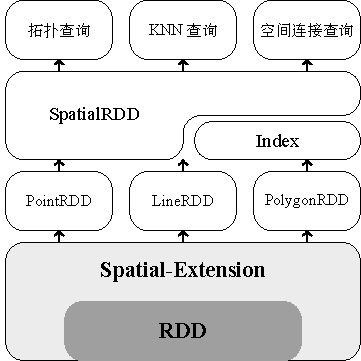
\includegraphics{figures/spatialspark.pdf}\\
  \caption{Spatial-Spark体系架构}{Spatial-Spark architecture}
  \label{fig:spatialsparkarchitecture}
\end{figure}

空间数据类型是Spatial-Spark的核心,通过RDD将点、线和面分别封装成PointRDD、LineRDD和PolygonRDD。这些Spatial-RDD表
示在集群中并行分区存储空间几何对象的集合,主要有两种方式生成Spatial-RDD:\circled{1}从HDFS中读取数据,主要流程见图\ref{fig:spatialrdd},文本空间
数据以行记录存储在HDFS中,先经过文件格式装换,将WKT,GeoJSON等数据转换成空间对象,再空间数据坐标参考系统转换统一,最
后生成Spatial-RDD,其中转换和投影步骤以接口形式提供,用户可以重写接口,完成定制化需求;\circled{2}Spatial-RDD相互之间空间运算,如PointRDD
可以通过缓冲区操作生成PolygonRDD对象,PolygonRDD对象通过提取重生成PointRDD。
\begin{figure}
\centering
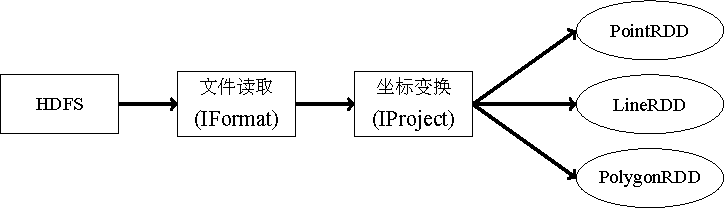
\includegraphics[scale=0.9]{figures/spatialRDD.pdf}
\caption{HDFS生成Spatial-RDD流程}{Generating Spatial RDD from HDFS} 
\label{fig:spatialrdd}
\end{figure}


\subsection{空间数据索引}
\subsubsection{RDD分区}
RDD内部数据集合在逻辑上(以及物理上)被划分为多个小集合,这样每个小集合就被成为分区。以图\ref{fig:rddpartition}为例,
RDD1有五个分区(Partition),分布在四个DataNode上面,而RDD2有三个分区,分布在
三个DataNode上面。在源码级别,RDD类存储一个Partition列表,每个Partition对象都包含
一个index成员,通过RDD编号加index就能从唯一的分区的Block编号\cite{Zaharia2012Resilient},持久化的RDD就能通过这
个Block变化从HDFS中获取对应的分区数据。
\begin{figure}
\centering
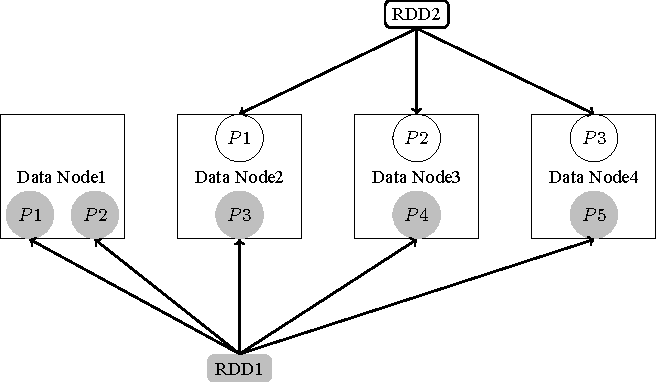
\includegraphics[scale=0.8]{figures/rddpartition.pdf}
\caption{RDD分区}{RDD partition illustration}
\label{fig:rddpartition}
\end{figure}

分区的个数决定了并行计算的粒度,多个分区能够并行计算,充分利用分布式计算资源。通常来讲,分区
的数量为计算集群的CPU核心数量的$3-4$倍。创建分区的方法主要有两种:\circled{1}在SparkContext对象读取数据
的时候指定分区的数量;\circled{2}调用RDD的分区器函数,进行重新分区。Spark在读取数据时默
认使用哈希分区器,该分区器实现简单,运算速度快,但缺点是不关心键值的分布情况,其散列到不同分区的概率会
因数据而异。往往会带来分区负载的不平衡性。

考虑到空间数据空间分布特点,Spatial-Spark提供了空间分区,重写了Partitioner函数,能够尽可能
将空间上分布相邻的空间对象处于同一RDD分区。具体算法步骤如下:

(1)根据空间要素集合的边界(boundary)和分区数量n,将整个boundary划分为$\sqrt{n}\times \sqrt{n}$个
网格,每个网格拥有一个id值。

(2)将\verb|RDD<Geometry>|进行Map或者MapPartition操作,使之转换为PairRDD<Integer,Geometry>描述
的Key-Value对象,其中Key为网格中与其相交或者包含的网格的id值,如果有多个网格与之相交,取其中一个。

(3)对\verb|PairRDD<Interger,Geometry>|按照key进行重分区计算,使每个分区能够拥有分布较为均匀的
几何对象,而且尽量保证相邻的空间的对象在同一个分区。

\subsubsection{分区索引}

好的空间索引能够极大地方便海量空间数据查询,而空间数据中最常用的空间数据索引方式就是R树。R树索引是有
美国加州大学Guttman A.教授提出的一种空间数据库的动态索引算法\cite{Guttman1984R},该数据结构的核心思想是通
过最小外包矩形(Minimum Bounding Rectangle, MBR)表达一个或者一组空间几何对象。与B树一样,R树是一棵高度平衡树,
将所有的空间几何对象都存放在叶节点,插入和删除节点不需要完全重构R树,只需要在局部进行相关拓扑调整即可,
一棵典型的R树如图\ref{fig:rtree}所示。
\begin{figure}
\centering
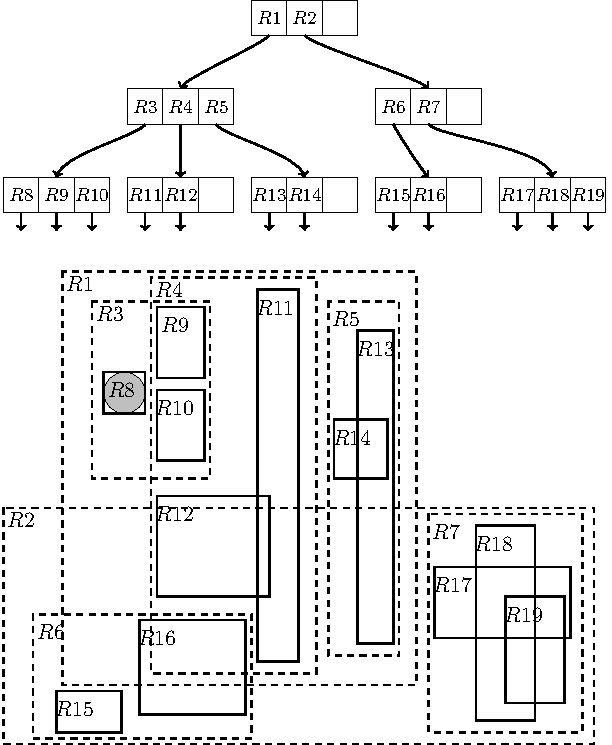
\includegraphics[scale=0.8]{figures/rtree.pdf}\\
\caption{R树示意图}{R tree illustration}
\label{fig:rtree}
\end{figure}

(1)R树插入

作为B树的一个变种,R树的插入与B树相类似,首先根据待插入空间对象的最小外包矩形待确定插入的叶节点,
然后插入对象,如果该叶节点包含的空间对象数目超过规定的最大数目,则将该节点进行分裂\cite{Huang2001Optimizing},并
将其中的一个节点向上传递,递归执行,如果直至根节点,完成树高度的提升。节点分裂的好还的标准是两个新节点的最小外包
矩形的面积之和最小。

(2)R树查询

R树查询只能检索出与给定窗口相交的空间实体对象。如果两个最小外包矩形是分离的,那么他们所代表的空间实体也肯定
是分离的,但如果两个最小矩形有相交,不能保证所包含的空间几何实体能够窗口相交。因此,R树空间检索检索策
略是:

过滤:从R树中筛选出候选节点,排除那些的不能满足相交条件的几何对象,但在候选几何对象中也
可能包含一些不满足条件的对象。由于判断最小外包矩形是否相交的计算成本低,可大幅度提高计算效率。

精选:依次判断每个候选几何对象,判断与查询窗口是否相交。可以借助JTS Topology Suite工具判断几何对象之间的拓扑关系。

在Spatial-Spark框架中,为了加快空间分析的速度,可选择在RDD的每个分区建立R树空间索引。通过RDD的MapPartition函数
将同一分区的空间对象汇集起来,每个分区建立一棵R树,将同一分区的几何对象的最小外包矩形插入树中。
通过Spark缓存机制,将索引内容缓存到Spark内存中,方便后续查询分析等工作。

\subsection{空间数据查询}

空间查询是GIS中最重要组成部分,在大规模空间数据中查询也提出了空间数据查询实时性要求。Spatial-Spark
在Spatial-RDD上层提供了空间查询层,包括空间拓扑查询(Spatial Topology Query),空间k邻居
查询(Spatial k Nearest Neighbor Query)和空间链接查询(Spatial Join Query)。使用者向
查询层发起空间查询请求,Spatial-Spark将查询的结果返回。如果空间数据在Spatial-RDD层事先建
立的了索引,那么用户可以借助索引,提高查询速度。

\subsubsection{空间拓扑查询}
空间拓扑关系是空间分析的特色,空间拓扑查询过程是给定一个空间几何对象和空间拓扑关系条件,从特定的
空间数据集筛选出符合条件的空间数据。

平面空间实体对象引入空间实体外部、内部和边界,构成了空间实体的基本组件。假设空间实体$A$的边界$\partial A$,
内部为$A^{\circ}$,补为$A^{-}$,空间实体$B$的边界为$\partial B$,内部为$B^{\circ}$,补为$B^{-}$,两两的交集就构
成了空间关系描述的9元组矩阵\cite{谢俊平2012拓扑关系和方向关系的统一表达模型}。
\[ R(A,B) = 
\begin{bmatrix}
\partial A \cap \partial B & \partial A \cap B^{\circ} & \partial A \cap B^{-} \\
A^{\circ} \cap \partial B & A^{\circ} \cap B^{\circ} & A^{\circ} \cap B^{-} \\
A^{-} \cap \partial B & A^{-} \cap B^{\circ} & A^{-} \cap B^{-} \\
\end{bmatrix}
\]

矩阵中每一个元素的取值都有空集和非空集两种,9个元素共存在512中可能,当然其中绝大部分
的空间拓扑关系时不存在的。以点、线和面为准给出所有可能空间对象之间可能拓扑关系,见表\ref{tab:geometrytopo}。
\begin{table}
  \centering
  \caption{空间几何拓扑关系}{Geometry topology rules}
  \label{tab:geometrytopo}
  \tabulinesep=1.5mm
  \begin{tabu}to 0.7\linewidth{X[1, c]X[1.2,c]X[1.2,c]X[1.2,c]}
    \tabucline[0.10em]-
    几何对象 & 点 & 线 & 面 \\
    \tabucline-
    点 & Equal\par Disjoint & Within\par Disjoint & Within\par Touch\par Disjoint \\
    \tabucline-
    线 & Contain\par Disjoint & Equals\par Within\par Overlap\par Contain\par Disjoint\par Intersect\par 
      & Within\par Disjoint\par Touch\par Intersect \\
    \tabucline-
    面 & Contain\par Disjoint & Contain\par Disjoint\par Touch\par Intersect\par &
    Equal\par Within\par Disjoint\par Touch\par Intersect\par Overlap\par Contain\par \\
    \tabucline[0.10em]-
  \end{tabu}
\end{table}

RDD中的filter算子可以筛选RDD中符合条件的元素,Spatial-Spark实现了Function接口的
通用空间拓扑查询类。该类接受待查询的空间元素Geometry和待判断的空间拓扑关系条件Condition。在
类中重写call函数即可,通用实现如下。
\begin{lstlisting}[language=Java]
@Override
public Boolean call(Geometry goe){
    return geo.condition(this.query)
}
\end{lstlisting}


当在Spatial-RDD中如果已经在每个分区构建好R树索引,可以通过索引查询相交(Intersect)、包
含(Contain)、相等(Equal)、重叠(Overlap)和被包含(Within)的拓扑关系。RDD中的FlatMapPartition算子
可以对每个分区进行操作,并将结果展平(Flat)返回,用户定义Spatial-Spark预先实现了FlatMapFunction接
口的类,该类构造函数只包含带查询对象的最小外包矩形(Envelope),通过R树高效的查询函数返回最小外包矩形与待查询
的外包矩形的空间几何对象。索引查询是初步空间查询,在返回的结果中,在对数据进行精确空间拓扑查询,通用实现如下。
\begin{lstlisting}[language=Java]
@Override
public Iterator<Geometry> call(Iterator<STRTree> t){
    STRtree tree = t.next()
    return tree.query(this.query.getEnvelopeInternal())
}
\end{lstlisting}

\subsubsection{空间k邻居查询}
空间K个近邻居查询在现实生活中有着广泛应用,尤其在移动互联网时代,位置推荐、商场选址和公共交通等方面有着
广泛应用\cite{董亭亭2013大数据下空间数据索引和}。Spatial-Spark在K邻居查询,算法借助优先级队列数据结构,
算法主要分为两步:\circled{1}选择:针对每个分区,接受一个查询点和查询邻居数量K,在该分区中,构建一个容量
为K的优先级队列,依次将计算查询点与分区内几何对象的空间欧氏距离,并添加至优先级队列中,如果队列已满,将
集合中距离最大元素删除再添加;\circled{2}合并:针对每个分区的优先级队列,再次筛选出前K个最小距离的几何
要素,KNN通用查询类如下。
\begin{lstlisting}[language=Java]
@Override
public Iterator<Geometry> call(Iterator<Geometry> inputs){
        while(inputs.hasNext()){
            if(pq.size()< this.k){
                pq.offer(inputs.next());
            }else{
                Geometry geo = inputs.next();
                double distance = geo.distance(this.query);
                double longestDistance = pq.peek().
                                    distance(this.query);
                if(longestDistance > distance){
                    pq.poll();pq.offer(geo);
                }
            }
        }
}
\end{lstlisting}


\subsubsection{空间连接查询}
空间连接查询是常用且复杂的空间数据查询操作,类似于数据库的两张表Join查询,从两个空间对象集合中查询出符合特定空间关
系的空间几何对象对\cite{Jacox2007Spatial}。例如两个空间数据集A和B,空间连接是从A中的空间对象到B中的空间对象使用空间拓扑
关系$t$,返回分别来自A和B的满足条件的几何对象对,空间对象的复杂性和海量性将会导致空间连接运算需要大量的
计算,时间复杂急剧上升。Spark的并行计算特点为空间连接运算提供了新的模式,因此Spatial-Spark采用了并
行化方式实现了空间连接查询算法。算法的主要步骤分为两步。

(1)过滤步骤

借鉴Spatial-Spark空间分区算法,首先将其中任意空间数据集的边界按其最小的几何对象外包
矩形分割成规则的网格,每个网格赋予编号。将空间数据集的每一个元素与判断与之相交的最小外包矩形
编号,通过RDD相应的MapToPair操作转换成PairRDD,其中键key为网格的编号,值value为空间几何对象,再使
用转换函数cogroup,按照key将连个要素集合并起来。
\begin{figure}
\centering
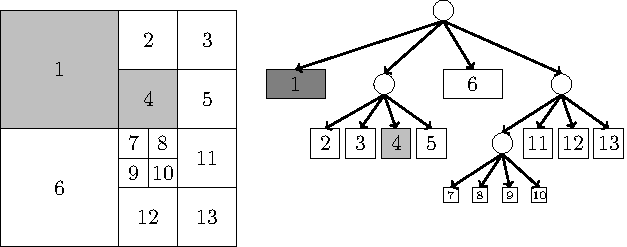
\includegraphics[scale=0.8]{figures/quadtree.pdf}
\caption{四叉树示意图}{Quadtree illustration}
\label{fig:quadtree}
\end{figure}


在空间元素最小外包矩形与格网相交时,可以预先将整个格网数据进行预处理。四叉树也是一种树状索引数据
结构,地理空间对象局部范围信息可以用四叉树进行存储,其采取从整体到局部划分的方式建立索引。建立过程
如下:对空间范围平面平均分成四个部分,如果改部分的空间对象属性一致,则不再划分,否则继续划分四个小
部分,如此重复递归执行。每划分一次,四叉树深度增加1,对于深度为$n$的四叉树索引,包含的空间对象至多为($2^n \times 2^n$)个,
四叉树示意图见\ref{fig:quadtree}。

对于空间连接查询中预先处理的格网建立的四叉树索引,所有的叶节点的深度相同,平均每次查询的时间复杂
度为$\log_{4}n$,而遍历整个格网的时间复杂度为$n$。

(2)求精步骤

在过滤阶段中,同一网格内空间对象,再根据空间拓扑要求精确筛选,返回结果中每个元素表示
一对满足条件的空间拓扑要求的几何对象对,整个空间连接过程见算法\ref{alg:join}。
\begin{algorithm}[h]   
\caption{空间连接查询}
\label{alg:join}
\begin{algorithmic}[1] %这个1 表示每一行都显示数字  
\REQUIRE  ~~\\ %算法的输入参数:Input  
空间RDD1:spatial\_rdd1;\\  
空间RDD2:spatial\_rdd2;\\  
\ENSURE ~~\\ %算法的输出:Output  
空间连接对象对, spatial\_join; \\
\STATE $//$与网格相交生成key-value;
\STATE spatial\_pair\_rdd1 = spatial\_rdd1.flatToPair(); \\ 
       spatial\_pair\_rdd2 = spatial\_rdd2.flatToPair();
\STATE $//$按key进行cogroup操作;

\STATE spatial\_pair\_groups = spatial\_pair\_rdd1.cogroup(spatial\_pair\_rdd2);

\STATE $//$每个value进行详细拓扑判断

\STATE spatial\_pair\_values = spatial\_pair\_groups.mapValue();  

\STATE $//$去重操作 
\STATE spatial\_pair\_join = spatial\_pair\_values.reduceByKey(); 
\STATE $//$去掉key 
\STATE spatial\_join = spatial\_pair\_join.mapToPair(); 
\RETURN spatial\_join; %算法的返回值  
\end{algorithmic}  
\end{algorithm} 


\section{Spatial-Spark实验分析}{Experiments and Analysises of Spatial-Spark}

\subsection{实验平台及配置}
为了验证Spatial-Spark计算框架在空间数据分析中的优势,搭建了Hadoop/Spark计
算集群\cite{Ghosh2017Install1, Ghosh2017Install2},整个集群有$10$台服务器组成,
每台服务器安装了VMware虚拟机,每台虚拟机使用的操作系统为Centos $6.4$ Linux操作
系统,每台虚拟机的配置见表\ref{tab:clusterconfig}:
\begin{table}
  \centering
  \caption{集群配置}{Cluster configurations}
  \label{tab:clusterconfig}
  \tabulinesep=1.5mm
  \begin{tabu}to 0.5\linewidth{X[1, c]X[1,c]}
    \tabucline[0.10em]-
    项目 & 配置  \\
    \tabucline-
    内存 & $4$G \\
    CPU核心 & 双核四线程 \\
    硬盘容量 & $30$G \\
    操作系统 & CentOS $64$位 \\
    Hadoop版本 & $2.6$ \\
    Spark版本 & $1.4$ \\
    JDK & $1.7$ \\
    以太网络 & $1000$Mbps \\
    \tabucline[0.10em]-
  \end{tabu}
\end{table}

Hadoop/Spark集群部署繁琐,涉及到各个方面的技术,其中包括Linux系统的配置,Hadoop的配置与
调试,Java和Scala语言库的安装,Spark计算框架配置和部署。 为了能够使集群能够相互通信,对
$10$台服务器IP地址划分和Hostname修改,因为集群之间需要进行数据交换处理,所以要配置使节点之
间能够SSH免密码通信。各节点IP配置见表\ref{tab:ipclusterconfig}:
\begin{table}
  \centering
  \caption{节点IP}{Nodes' IP addresses}
  \label{tab:ipclusterconfig}
  \tabulinesep=1.5mm
  \begin{tabu}to 0.8\linewidth{X[1,c]X[1,c]|X[1, c]X[1,c]}
    \tabucline[0.10em]-
    节点 & IP地址 & 节点 & IP地址  \\
    \tabucline-
    Master & $192.168.5.100$ & Node$5$ & $192.168.5.105$ \\
    Node$1$ & $192.168.5.101$ & Node$6$ & $192.168.5.106$ \\
    Node$2$ & $192.168.5.102$ & Node$7$ & $192.168.5.107$ \\
    Node$3$ & $192.168.5.103$ & Node$8$ & $192.168.5.108$ \\
    Node$4$ & $192.168.5.104$ & Node$9$ & $192.168.5.109$ \\
    \tabucline[0.10em]-
  \end{tabu}
\end{table}

其中Master节点为主节点,守护Hadoop的Namenode进程、Yarn的ResourceManager进程和Spark的
Master进程。而Node$1\sim $Node$9$节点为从节点,守护Hadoop的Datanode进程和Spark的Worker进程,其
中Node1节点另外守护Hadoop SecondaryNameNode进程,当Master节点的Namenode进程出现
故障,Node$1$节点将被担当起NameNode节点的作用。

Spark计算模式主要分为三种:Local模式、Standalone模式和Yarn-Cluster模式。Local模式是在
本地运行,Spark的Local模式部署简单,适合单机上调试编写的Spark 应用程序;Standalone模式
是Spark自身实现资源调度框架\cite{Fern2016Automated},当不需要其他计算框架的时候如MapReduce、Storm等,只使用
Spark进行大数据计算时,可以采用Standalone模式,其中Spark Shell交互式运行环境就是运行在
该模式之上;Yarn-Cluster模式借助Yarn统一管理整个计算资源,用户在Yarn集群中的服务和Spark
应用的资源完全隔离。

为了方便调试,本实验采用Standalone模式,当整个集群配置完毕后,启动Spark-Shell,采用Scala
交互式语言编写WordCount程序,返回正确结果表明整个hadoop-spark集群配置成功。
\subsection{实验对比分析}

(1)MapReduce与Spatial-Spark空间过滤筛选对比

在相同的集群中,分别编写MapReduce应用程序和Spatial-Spark应用程序,对相同规模的空间数据进
行空间数据分析。选用的数据为全国所有道路线状空间对象(包括高速公路、国道、省道、县道),首先
对原有的ShapeFile数据转换成OGC标准的WKT文件,按行存储为一个空间对象,在集群中通过Hadoop相关命
令,存放到HDFS中,集群中HDFS的Block的大小为$128$M。空间过滤算法定义为选择其中一条道路,求解
其外包矩形中包含的所有其他道路。

实验分为五组,实验数据量分别为$200$M、$500$M、$1$G、$2$G和$3$G,结果见图\ref{fig:topycomparsion},当数据量不大的
时候,Spatial-Spark相对于MapReduce优势不够明显,当数据量达到一定程度后,Spatial-Spark内存
计算的优势突显出来,在相同的条件下,MapReduce消耗的时间是Spatial-Spark的两个数量级。
\begin{figure}
  \centering
  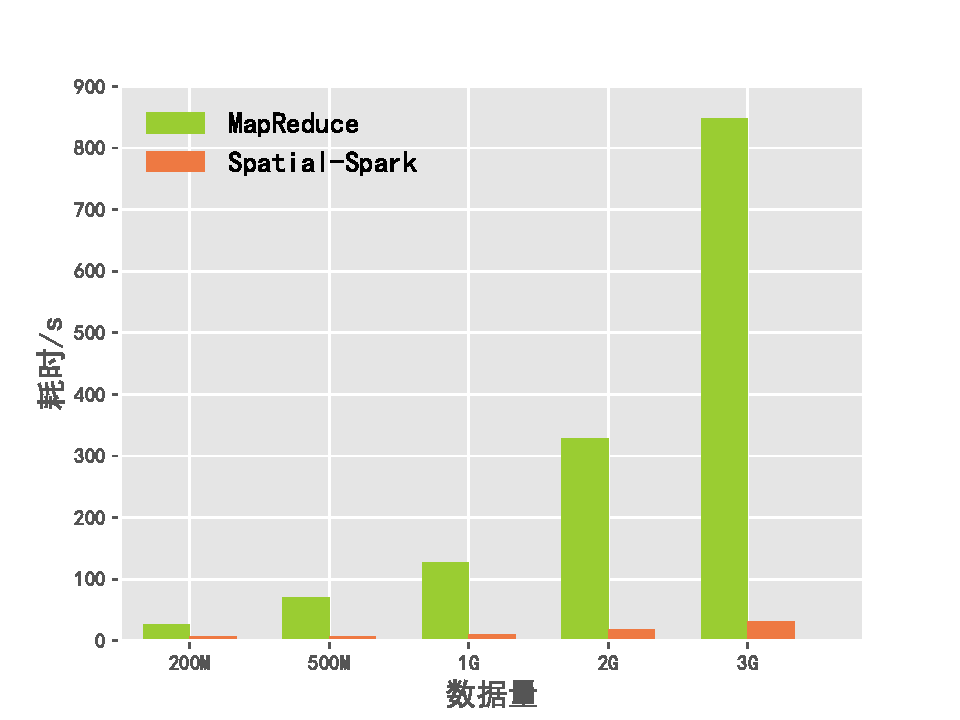
\includegraphics[scale=0.7]{figures/topo_query.pdf} \\
  \caption{MapReduce和Spatial-Spark查询对比}{MapReduce and Spatial-Spark topology query comparsion}
  \label{fig:topycomparsion}
\end{figure}

(2)Spatial-Spark集群扩展性能分析

Spatial-Spark计算框架的优越性在于其横向扩展性(Scale Out),通过增加廉价的计算机,使得
计算性能呈现显著性增加。在空间大数据分析中也不例外,本实验通过分析动态调整工作节点的
数目,比较在相同的数据规模下各个不同工作节点数目下,消耗的时间对比。

空间连接查询是空间运算中计算量较大的运算,选用的数据为全国县界面对象,共2917个面对象,与
全国道路中进行连接操作,获取每个县与之相交的道路。

实验共分为四组,使用的Work Node的数量分别为$2$、$4$、$6$和$8$,实验数据量$150$M县界对象,$1$G的全国道
路。为实验结果见图\ref{fig:node_memory},第一组实验引发java.lang.OutOfMemoryError异常,集群内存不足。其余
实验组时间消耗大致相同。

内存大小也是影响Spatial-Spark运算速度中重要因素,Spark在提交任务时候,可以通过executor-memory参数指
定每个工作节点提供给本次计算的内存,Standalone工作模式将会统一管理这些内存和资源调配。通过调整
内存参数,分析空间链接操作耗时。
\begin{figure}
  \centering
  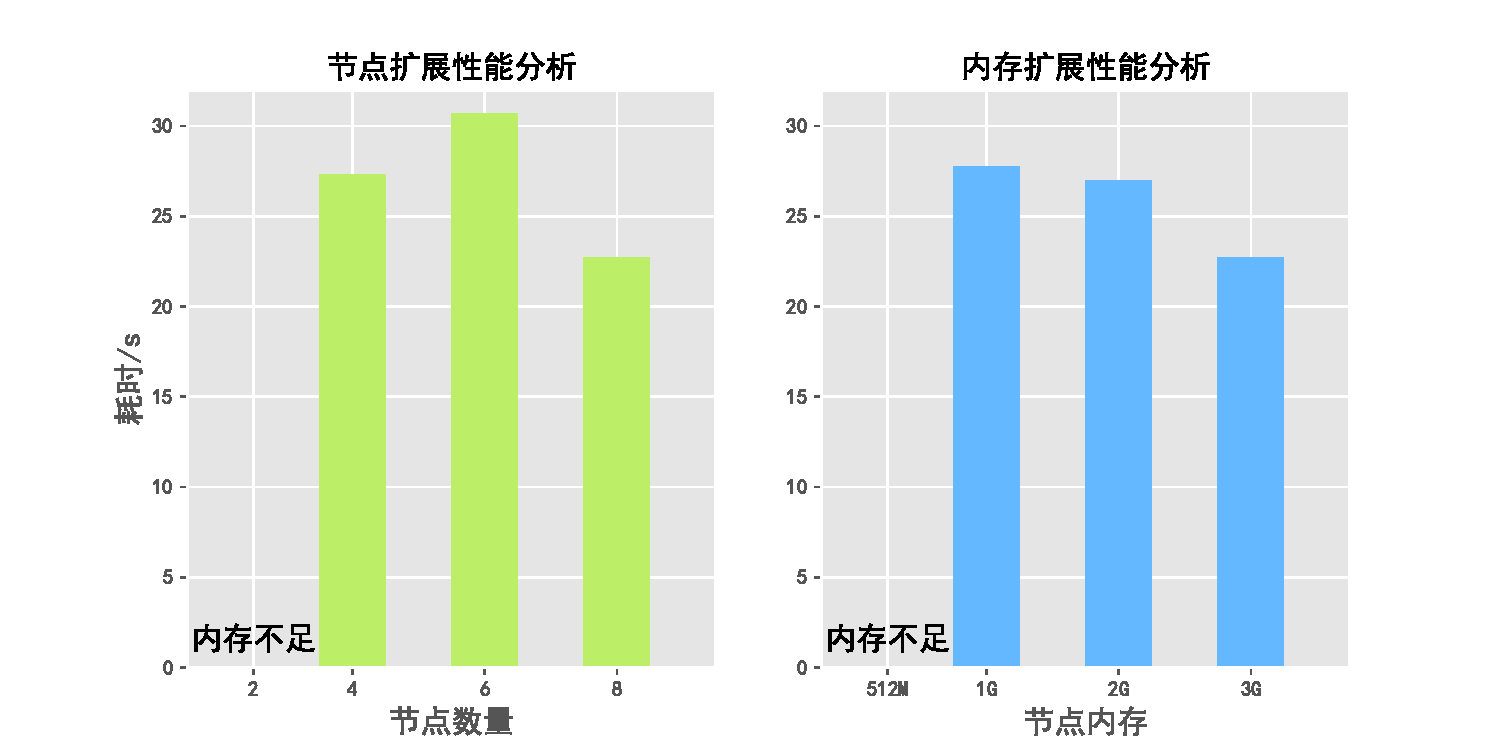
\includegraphics[scale=0.5]{figures/node_memory.pdf} \ \
  \caption{Spatial-Spark扩展性实验}{Spatial-Spark scale-out results}
  \label{fig:node_memory}
\end{figure}

实验共四组,每一组节点的内存分别为$512$M、$1$G、$2$G和$3$G,实验数据量$150$M县界对象,$1$G的全国道路。实验结
果见图\ref{fig:node_memory},第一组实验引发java.lang.OutOfMemoryError异常,集群内存不足。其余实验随着集群内存
的增大,时间消耗也呈下降趋势。

(3)Spatial-Spark空间索引性能分析

Spatial-Spark不仅仅是RDD的空间拓展,而且在分布式空间计算中引入了空间索引,并将索引通过Spark存
储策略缓存在内存中,并根据空间数据的分区,为每个分区建立了索引。由于R树索引存储的为空间对象的最
小外包矩形,因此在相关空间分析时,需要在初步筛选后进行精确空间判断分析。
\begin{figure}
  \centering
  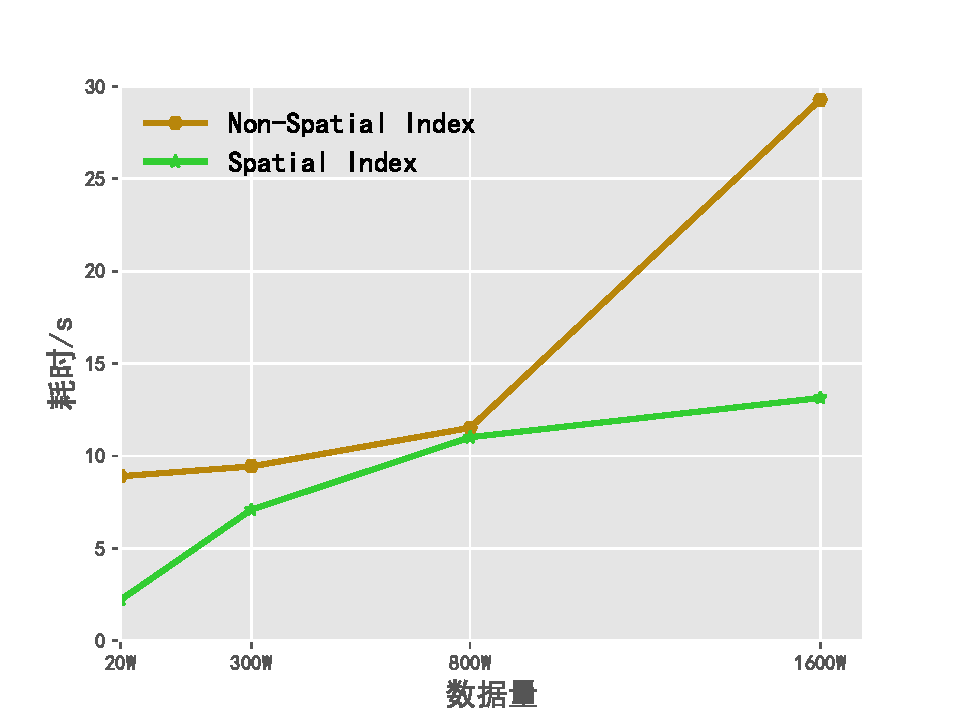
\includegraphics[scale=0.7]{figures/index.pdf} \\
  \caption{Spatial-Spark索引和非索引比较}{Spatial-Spark index Vs. non-index query comparsion}
  \label{fig:index}
\end{figure}

KNN空间查询是常用的空间数据查询分析,选择全国兴趣点(POI)共八百多万条数据,共$2.3$G,按行存储
数据,包含了空间和非空间数据。

实验总共分为四组,POI数目分别为$20$W、$300$W、$800$W和$1600$W,结果见图\ref{fig:index},对已经建立空间索引的KNN
查询消耗时间比非空间索引少,随着数据量增加,空间索引优势越发明显。
\subsection{Spatial-Spark优化方案}

Spark程序都具有「内存计算」的天性,所以集群中的所有资源:CPU、网络带宽或者内存都是成为Spark程序性能的瓶颈。

(1)数据序列化

序列化的作用是能够将数据在集群网络传输,因此序列化的对于提高分布式程序的性能起到重要的作用,一个不
好的序列化方式将会极大地降低计算速度。因此优化对象的为提高Spark应用程序的第一选择\cite{Zhao2016An}。Spark提供
了两种序列类库: \circled{1} Java序列化:在默认情况下,Spark采用Java的ObjectOutputStream序列化一个对象,只要
类实现了java.io.Serializable接口。Java序列化十分灵活方便,但是速度较慢;\circled{2}Kryo序列化:Spark也
能使用Kryo序列化对象,Kryo不仅速度快,而且生成的结果更为紧凑。但Kryo序列化使用比较繁琐,需要提
前注册要序列化的类。

在Spatial-Spark中,实验表明使用Java序列化对象某一RDD消耗为$434$M内存,当改用Kryo序列化后占该
RDD消耗$53$M内存,优化效果明显。

(2)内存优化

Spark内存计算给大数据分析带来了便利,但针对特别大的分析数据,内存无法完整加载,RDD持久化API提
供了多种序列化存储级别,见表\ref{tab:level},不同的序列化选择,使得在处理大数据时在效率和内存之间选择不同的权衡。

\begin{table}
  \centering
  \caption{存储级别策略}{Storage level stragies}
  \label{tab:level}
  \tabulinesep=1.5mm
  \begin{tabu}to 0.8\linewidth{X[1, c]X[1,c]}
    \tabucline[0.10em]-
    存储级别 & 说明  \\
    \tabucline-
    MEMORY\_ONLY & 全部序列化到内存 \\
    DISK\_ONLY & 全部序列化到磁盘 \\
    MEMORY\_AND\_DISK & 序列化到内存和磁盘 \\
    MEMORY\_ONLY\_SER & 序列化到内存字节数组 \\
    \tabucline[0.10em]-
  \end{tabu}
\end{table}

用多大内存来缓存数据是内存回收是非常重要的参数,在默认情况下,Spark采用运行内存
的$60\%$空间来进行RDD缓存,所以在程序运行期间只有$40\%$的内存可以用来创建对象。当程序运行过程中JVM频
繁进行垃圾回收,会大大减低程序运行速度,为了提高效率,可以手动修改缓存大小比例。

\section{本章小结}{Chapter Summary}

本章着重介绍了Spatial-Spark大数据空间分析框架,首先分析了矢量空间数据格式种类,空间数据转换和开源空间
数据分析包;接着对Spark核心数据结构RDD空间扩展为Spatial-RDD,并着重对空间数据进行空间分区索引,
以此为基础,构建了常见空间分析应用API。以实验为基准,分析了Spatial-Spark的性能方面的特点。

\section{POI空间分析}

\subsection{POI获取}

\begin{frame}[c]{微博数据接口}
    新浪微博提供了API方便第三方程序访问微博丰富的数据资源

    \begin{figure}
        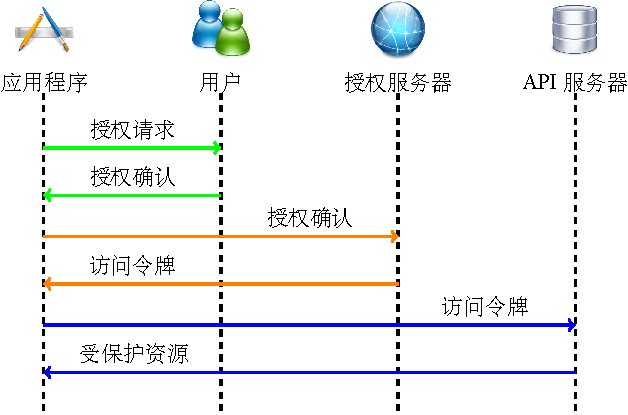
\includegraphics[scale=0.8]{figures/api.pdf}
    \end{figure}

    \pause
    \alert{HTTP Get}
\end{frame}

% \begin{frame}[t]{微博数据接口}
    

%     \vspace{0.5em}
%     \pause
%     \begin{itemize}
%     \item location/geo/address\_to\_geo $\rightarrow$  根据地址返回地理信息坐标 
%     \item location/pois/show\_batch $\rightarrow$ 批量获取POI点的信息
%     \item location/citycode $\rightarrow$ 城市代码对应表
%     \item place/nearby/pois $\rightarrow$ 获取附近的POI点
%     \end{itemize}
% \end{frame}

\begin{frame}[c]{POI空间分析(获取)}
    POI是新浪微博用户在使用过程中自行添加附近的热门位置

    \vspace{1em}
    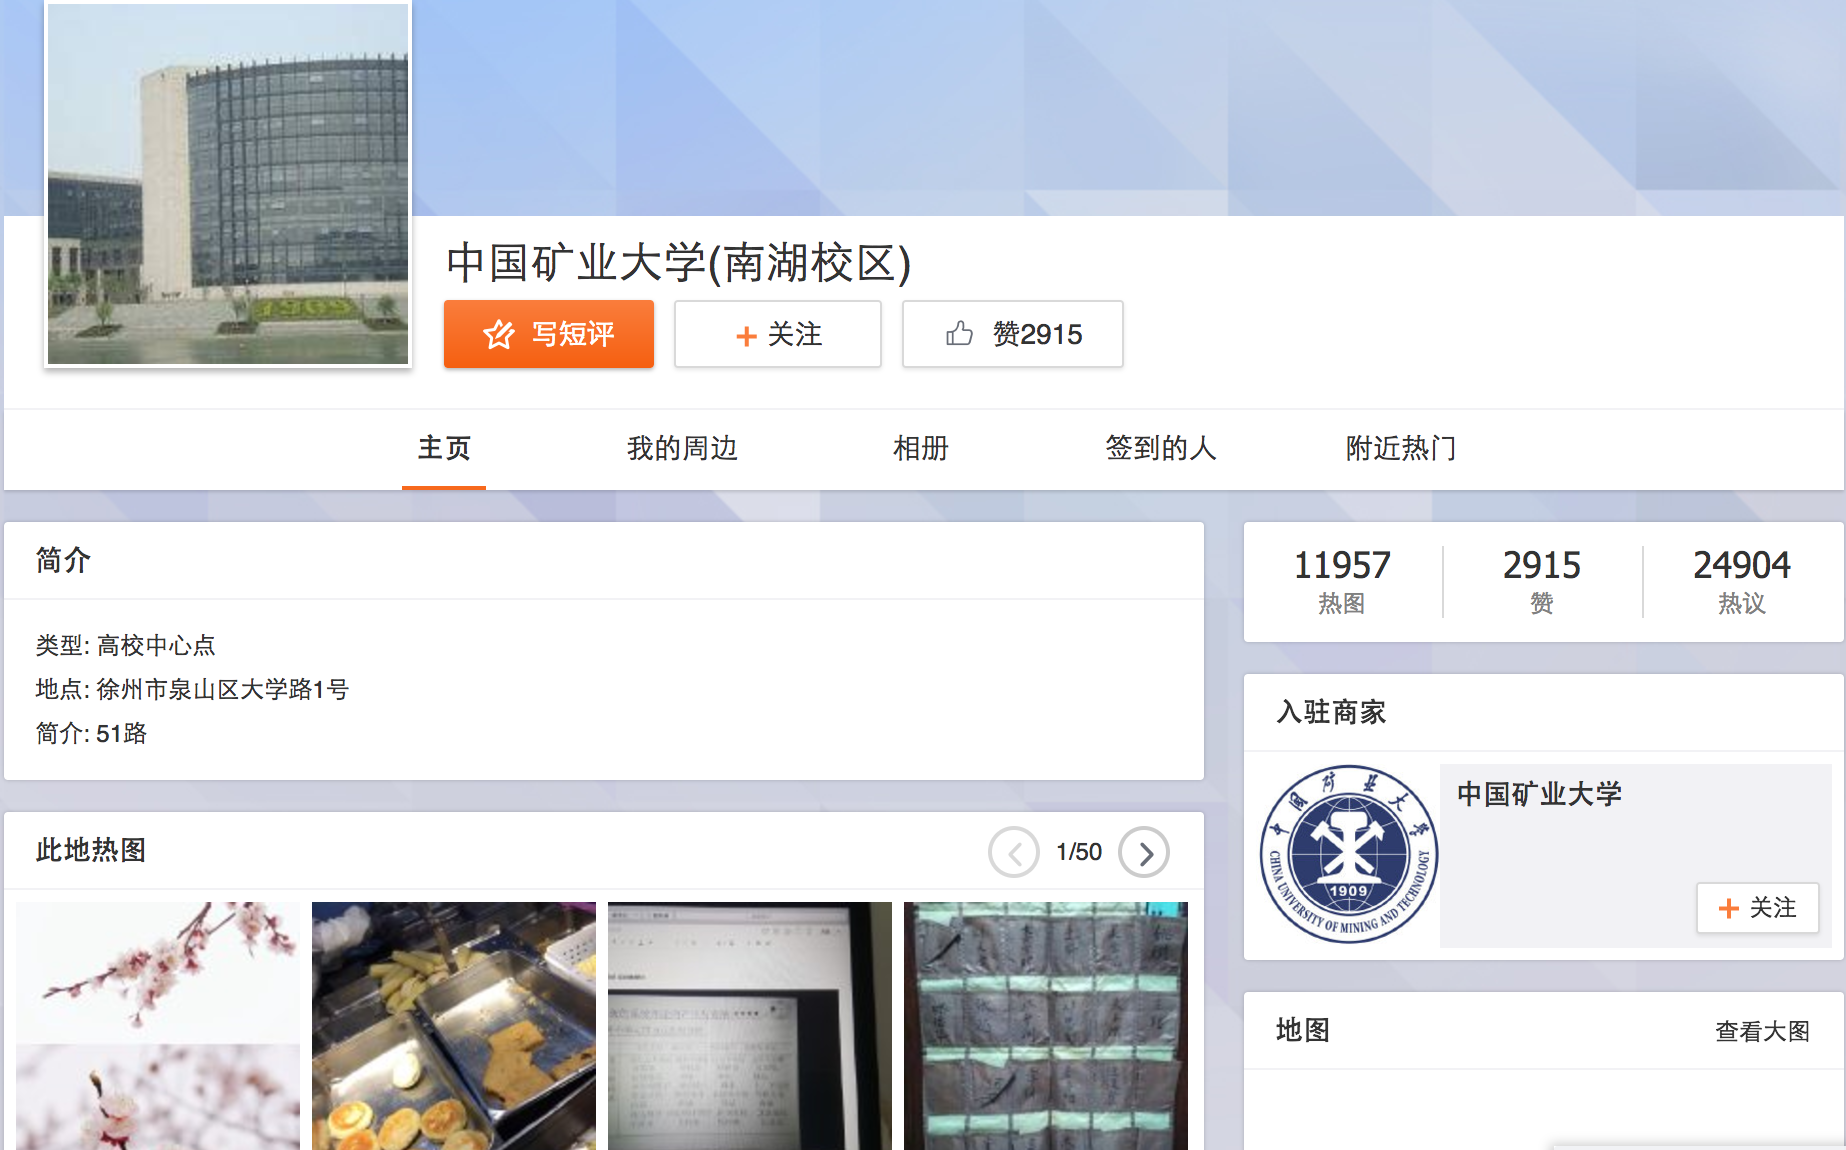
\includegraphics[scale=0.3]{figures/webpoi.png}
\end{frame}

\begin{frame}[c]{POI空间分析(获取)}
    \begin{columns}
        \begin{column}{0.5 \textwidth}
            \alert{place/nearby/pois}
            \vspace{1em}
            \begin{itemize}
                \item \textbf{Lat:} 纬度
                \item \textbf{Long:} 经度
                \item \textbf{Range:} 查询半径
            \end{itemize}
        \end{column}
        
        \pause
        \begin{column}{0.5 \textwidth}
            \begin{itemize}
                \item \alert{投影}

                Lambert 投影

                \pause
                \item \alert{栅格化}

                \vspace{0.5em}
                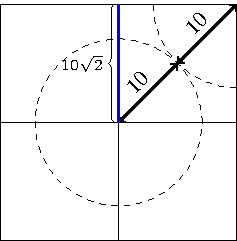
\includegraphics[scale=0.8]{figures/query.pdf}

                \pause
                \item \alert{坐标反算}

                适应API接口

            \end{itemize}
            
        \end{column}
    \end{columns}
\end{frame}

\subsection{统计分析}

\begin{frame}[c]{POI空间分析(统计)}
    \begin{columns}
        \vspace{0.5em}
        \begin{column}{0.5 \textwidth}
            \alert{热门签到地点}: sortBy, take

            \pause
            \begin{enumerate}
                \item 星光公益站
                \item 浦东机场
                \item 厦门高崎国际机场
                \item 中关村
                \item 深圳宝安机场
                \item 丽江古城
                \item 成都双流国际机场
                \item 望京
                \item 首都机场T3航站楼
                \item 广州白云机场
            \end{enumerate}
        \end{column}

        \pause
        \vspace{0.5em}
        \begin{column}{0.5 \textwidth}
            \alert{热门签到类别}: groupBy, reduce

            \pause
            \vspace{2em}
            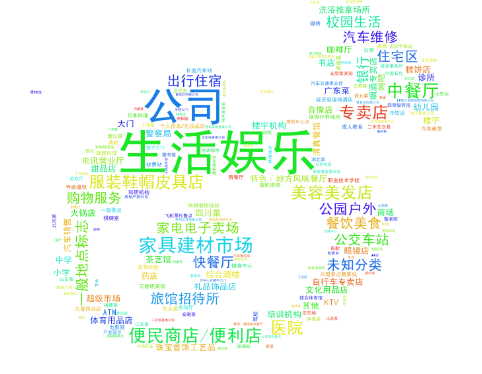
\includegraphics[scale=0.4]{figures/poi_category.png}
        \end{column}
    \end{columns}
\end{frame}



\subsection{同位模式}

\begin{frame}[c]{POI空间分析(同位模式)}
    \alert{关联规则算法}

    \vspace{1em}
    \begin{itemize}
        \item 事务项$T$,由集合$I_1,I_2,\ldots,I_m$组成
        \item $P \in T, Q \in T$,规则$P \rightarrow Q$
        \item 置信度约束 $c(P \rightarrow Q) \ge min\_c$
        \item 支持度约束 $s(P \rightarrow Q) \ge min\_s$
    \end{itemize}

    \pause
    \vspace{1em}
    \alert{Apriori算法}

    \begin{itemize}
        \item 频繁项的子 集必须也是频繁的
        \item 非频繁项的超集必定非频繁
    \end{itemize}
\end{frame}

\begin{frame}[t]{POI空间分析(同位模式)}

    \begin{alert}{单主题空间关联规则}
     \begin{equation}
        P_1\wedge P_2\wedge \ldots \wedge P_m \rightarrow Q_1\wedge Q_2\wedge \ldots \wedge Q_n(s\%, c\%)
    \end{equation}
    \end{alert}
    % % 单主题空间关联规则
    
    \pause
    \begin{alert}{多主题同位模式}
            \begin{equation}
                R(a_1,b_1) \Leftrightarrow (distance(a_1,b_1)\le d)
            \end{equation}

            \pause
            \begin{figure}
                \centering
                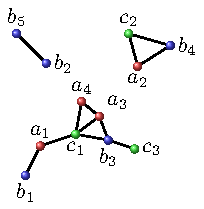
\includegraphics[scale=1.0]{figures/spatialrelation.pdf}
            \end{figure}
    \end{alert}

    % 其中$P_i$和$Q_j$中至少有一个为空间谓词
\end{frame}

% \begin{frame}[c]{POI空间分析(同位模式)}
%     多主题同位模式
%     \begin{equation}
%         R(a_1,b_1) \Leftrightarrow (distance(a_1,b_1)\le d)
%     \end{equation}

%     \pause
%     \begin{figure}
%         \centering
%         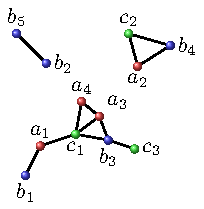
\includegraphics[scale=1.0]{figures/spatialrelation.pdf}
%     \end{figure}
% \end{frame}

\begin{frame}[c]{POI空间分析(同位模式)}
    \begin{columns}
        \begin{column}{0.3 \textwidth}
            \begin{figure}
                \centering
                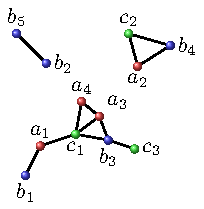
\includegraphics[scale=0.8]{figures/spatialrelation.pdf}
            \end{figure}
        \end{column}

        \begin{column}{0.7 \textwidth}
            \alert{参与率}
            \begin{equation}
                PR(c,f_i)=\frac{|\pi_{f_i}(table\_instance(c))|}{|table\_instance(\{f_i\})|}
            \end{equation}
            $PR(\{A,B,C\},A)=2/4=0.5$
            
            $PR(\{A,B,C\},B)=2/5=0.4$
            
            $PR(\{A,B,C\},C)=2/3=0.67$

            \pause
            \vspace{0.5em}
            \alert{参与度}
            \begin{equation}
                PI(c)=min_{i=1}^{k}\{PR(c,f_i)\}
            \end{equation}

            $PI(\{A,B,C\})=min(0.5,0.4,0.67)=0.4$
        \end{column}
    \end{columns}
\end{frame}

\begin{frame}[t]{POI空间分析(同位模式)}
    Spatial-Spark二阶模式生成

    \vspace{1em}
    \begin{figure}
        \centering
        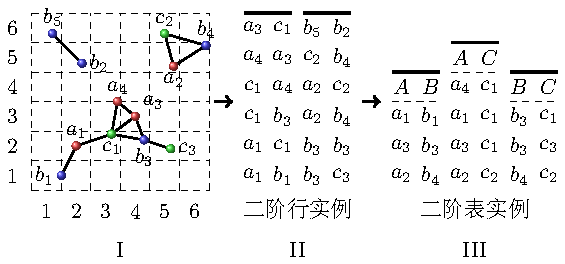
\includegraphics[scale=0.6]{figures/two_order.pdf}
    \end{figure}
    

    \pause
    键值相等判断
    \begin{figure}
        \centering
        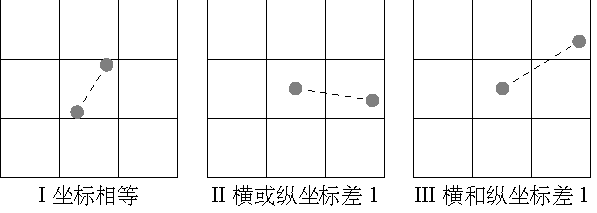
\includegraphics[scale=0.5]{figures/keyequal.pdf}
    \end{figure}
  
\end{frame}

\begin{frame}[t]{POI空间分析(同位模式)}

% \begin{algorithm}[H]
% \begin{algorithmic}[1]
% \FOR{$i=1$ to $N$}
% \FOR{$j=1$ to $JJJJ$}
% \STATE $energy[i*JJJ+j] =$ 
% $ interpolate(AAA[i*JJJ+j], ZZZ)$
% \ENDFOR
% \ENDFOR
% \end{algorithmic}
% \caption{pseudocode for the calculation of }
% \label{alg:seq}
% \end{algorithm}
\begin{algorithm}[H]
\tiny
\caption{co-location算法}
\begin{algorithmic}[1]   
\REQUIRE  ~~\\  
点集:points;\\  
距离阈值:d;\\
参与度阈值:threshold;\\  
\ENSURE ~~\\  
空间同位模式:colocation patterns; \\
\STATE $P_2$ = Spatial-Spark.join(points, d, threshold)
\WHILE{$P_k$ is not empty and $k$ < N} 
\pause
\STATE // \alert{Join操作,RowPattern重写}
\STATE $C_{k+1}$ = gen\_candinate\_cocolation($P_k$,$k$) $//$k+1阶候选集合
\pause
\STATE // \alert{距离阈值比较}
\STATE $C_{k+1}$ = pruning($C_{k+1}$, $d$)
\pause
\STATE // \alert{reduce生成表实例}
\STATE $T_{k+1}$ = gen\_table\_ins()$//$生成表实例
\pause
\STATE // \alert{threshold 筛选}
\STATE $P_{k+1}$ = Select\_Colocation\_Pattern($T_{k+1}$, threshold) $//$ 筛选表实例
\pause
\STATE $k$ = $k+1$ $//$下一轮迭代
\pause
\ENDWHILE 
\pause
\RETURN $P_2$,$\dots$,$P_k$
\end{algorithmic}
\end{algorithm} 
\end{frame}


\begin{frame}[c]{POI空间分析(同位模式)}
    \scriptsize
    \begin{columns}
        \begin{column}{0.333 \textwidth}
        \alert{上海市}

        \vspace{1em}
        (高等院校,校园生活):0.556

        \vspace{1em}
        (高等院校,日本料理):0.472

        \vspace{1em}
        (高等院校,西餐厅):0.454
        \vspace{1em}

        (高等院校,甜品店):0.451
        \vspace{1em}

        (高等院校,培训机构):0.446
        \vspace{1em}

        (高等院校,医院):0.443
        \vspace{1em}

        (高等院校,糕饼店):0.441
        \vspace{1em}

        (高等院校,餐饮美食):0.432
        \end{column}

        \begin{column}{0.333 \textwidth}
        \alert{武汉市}
        \vspace{1em}

        (高等院校,校园生活):0.531
        \vspace{1em}

        (高等院校,图书馆):0.528
        \vspace{1em}

        (高等院校,糕饼店):0.384
        \vspace{1em}

        (高等院校,快餐厅):0.368
        \vspace{1em}

        (高等院校,四川菜):0.361
        \vspace{1em}

        (高等院校,火锅店):0.358 
        \vspace{1em}

        (高等院校,连锁酒店):0.354
        \vspace{1em}

        (高等院校,医院):0.328
        \end{column}

        \begin{column}{0.333 \textwidth}
        \alert{重庆市}

        \vspace{1em}
        (高等院校,校园生活):0.306
        \vspace{1em}

        (高等院校,ATM):0.238
        \vspace{1em}

        (高等院校,科研机构):0.224
        \vspace{1em}

        (高等院校,图书馆):0.224
        \vspace{1em}

        (高等院校,超市):0.217
        \vspace{1em}

        (高等院校,特色餐厅):0.215
        \vspace{1em}

        (高等院校,电子卖场):0.210
        \vspace{1em}

        (高等院校,KTV):0.205
        \end{column}
        
    \end{columns}
\end{frame}

\begin{frame}[c]{POI空间分析(同位模式)}
    \alert{(高等院校, 培训机构)}

    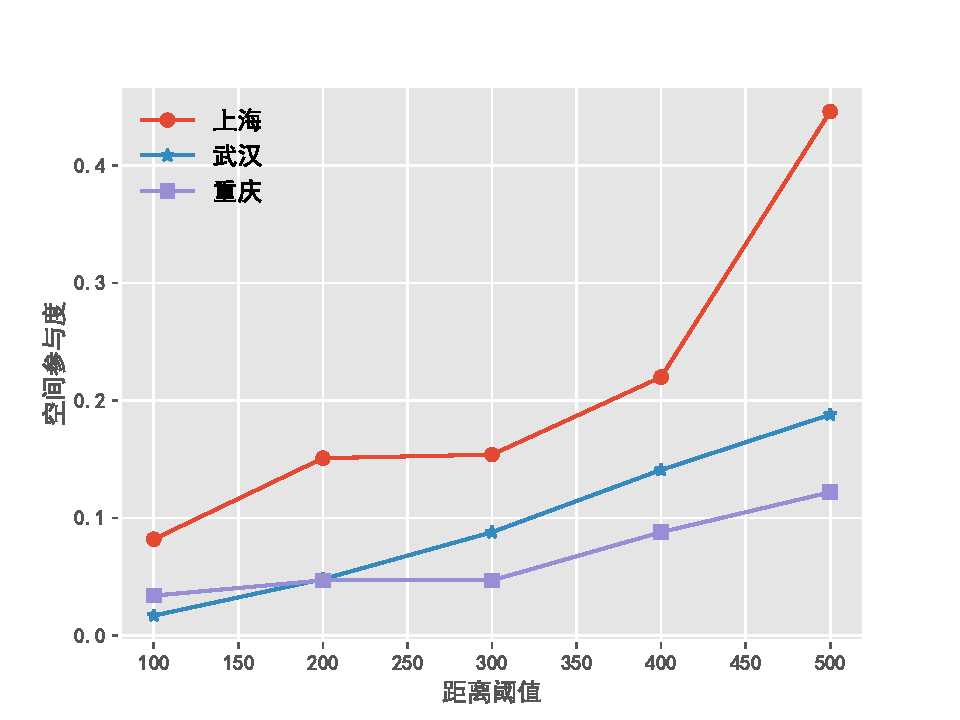
\includegraphics[scale=0.6]{figures/Participate.pdf}
\end{frame}

\begin{frame}[c]{POI空间分析(同位模式)}
    北京市POI空间模式,$d=500$m,空间参与度阈值为$0.6$

    \begin{itemize}
        \footnotesize
        \pause
        \item \textbf{二阶(29)}

        (中餐厅,校园生活),(校园生活,医院),(甜品店,中餐厅),(咖啡厅,校园生活),(咖啡厅,酒吧),(清真餐馆,酒吧) $\ldots$

        \pause
        \item \textbf{三阶(29)}

        (中餐厅,校园生活,医院),(电影院,KTV,美容美发店),
        (甜品店,中餐厅,美容美发店),(美容美发店,酒吧,甜品店),(中餐厅,校园生活,咖啡厅) $\ldots$

        \pause
        \item \textbf{四阶(19)}

        (电影院,KTV,咖啡厅,美容美发店),(KTV,中餐厅,甜品店,美容美发店),
        (甜品店,中餐厅,咖啡厅,美容美发店),(甜品店,咖啡厅,美容美发店,酒吧)$\ldots$

        \pause
        \item \textbf{五阶(7)}

        电影院,KTV,咖啡厅,甜品店,美容美发店),(KTV,中餐厅,咖啡厅,美容美发店,酒吧),
        (甜品店,中餐厅,咖啡厅,美容美发店,酒吧)$\ldots$

        \pause
        \item \textbf{六阶(1)}

        (KTV,中餐厅,咖啡厅,甜品店,美容美发店,酒吧)
    \end{itemize}
\end{frame}
\chapter{人口空间流动网络分析}{Analysis of Population Spatial Floating Network}
人口流动是直接塑造城市间关系的重要动力,也是城市发展活力指标\cite{甄峰网络社会}。城市之间的
人口流动研究始终是人文地理学、城市地理学和经济地理学所关注的热点。现代社会发展,交通网络的日趋
发达将城市发展与人口流动紧密地联系在一起,人口活动不再局限于一个封闭的城市。从全球、国家或区域
层面来看,人口流动已经跨越了地理的限制。传统的人口流动的统计方法费时费力,社交网络应用使用LBS功能
为研究这列问题提供了新思路,通过新浪微博提供的API接口获取特定时间段内全国范围内发送微博的用户,根据用户
的账户位置信息和发送微博的位置信息,构建基于社交地理的人口流动网络,如图\ref{fig:floatinpopulation}所示。
\begin{figure}
  \centering
  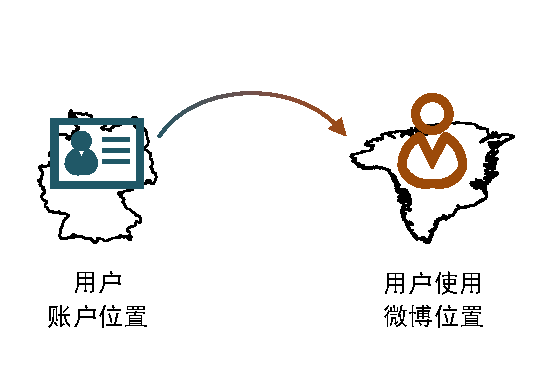
\includegraphics{figures/floating.pdf} \\
  \caption{流动示意图}{Floating illustration}
  \label{fig:floatinpopulation}
\end{figure}

\section{数据获取}{User Data Fetch}

新浪微博提供了place/nearby/users接口来获取附近发微博的用户,接口参数见表\ref{tab:poianduserapi}。
\begin{table}
  \centering
  \caption{NearbyUsers接口参数}{Nearby users api parameters}
  \label{tab:poianduserapi}
  \tabulinesep=1.5mm
  \begin{tabu}to 0.8\linewidth{X[1,c]X[1,c]X[2,c]}
    \tabucline[0.1em]-
    参数 & 类型 & 说明 \\
    \tabucline-
      lat & Float & 纬度 \\
      long & Float & 经度 \\
      starttime & Int64 & 开始时间 \\
      endtime & Int64 & 结束时间 \\
      range & Int & 查询半径,最大10km \\
    \tabucline[0.1em]-
   \end{tabu}
\end{table}

这些新浪微博用户数据包含了用户的名称、账号位置和用户当时所在空间位置,部分属性见格式见表\ref{tab:returnvalueuser}。
\begin{table}
  \centering
  \caption{用户地理空间位置(部分)}{Users' location information(partly)}
  \label{tab:returnvalueuser}
  \tabulinesep=1.5mm
  \begin{tabu}to 1.0\linewidth{X[1,c]X[2,c]|X[1,c]X[2,c]}
    \tabucline[0.1em]-
    属性 & 说明  & 属性 & 说明\\
    \tabucline-
    ID & 用户新浪微博ID & Name & 用户新浪微博名称 \\
    Province & 用户账户省份 & City & 用户账户城市 \\
    Lon & 用户位置经度 & Lat & 用户位置纬度\\
    \tabucline[0.1em]-
   \end{tabu}
\end{table}

春节前后是全国人口流动最为频繁的时间段,也是最能反映全国人口流动情况。因此选择$2016$年春节
前后$1$月$10$日和$2$月$10$日为起讫时间,获取全国微博用户位置数据,共$4.3$G,约$1500$万条用户记录。返回的数据为JSON格式,以键值的形式
保存表\ref{tab:returnvalueuser}中的属性,由于网络等其他问题,当请求量大的时候JSON数据中噪声较多,为了方便处理这些数据
因此将数据按行存放到HDFS中。

人口在不同城市之间流动构成了人口流动网络图,城市相当于网络图中节点,
不同城市之间人口流动相当于图中顶点之间的有向连接边,而人口流动数量则相当于边的权重。

GraphX作为Spark上层图处理模块,提供了并行化图分析算法。
为了方便分析城市人口流动分析,使用Spatial-Spark空间查询将全国数据抽象为一个Graph对象,
其中边$E_{ij}$为的权重为城市$j$中城市$i$用户的数量,算法流程图见\ref{fig:generateGraph}。
\begin{figure}
  \centering
  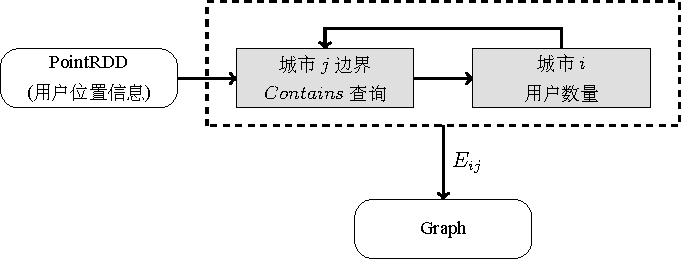
\includegraphics[scale=0.8]{figures/graph.pdf} \\
  \caption{Spatial-Spark生成人口流动网络图}{Generation floating population graph using Spatial-Spark}
  \label{fig:generateGraph}
\end{figure}

\section{人口流动统计}{Statistic of Floating Population}
\subsection{流动指数}

为了定量分析人口流动情况,定义如下指数:

\begin{description}
\item[流入量:]账户为其他城市在$i$城市发送微博的微博用户量,用$\delta_i$表示;
\item[流出量:]账户为$i$城市在其他城市发送微博的微博用户量,用$\omega_i$表示;
\item[流入流出比:]流入量/流出量,$\psi_i=\delta_i / \omega_i$。
\end{description}

\subsection{并行化设计}
GraphX丰富的图操作运算中\cite{Gonzalez2014GraphX},其中aggreateMessages是最核心最强大的接口,
该方法将边和其关联两个顶点作为一个Triplet进行整体并行处理,如图\ref{fig:triplet}所示,节点A和B以及它们之间的有向边
组成一个Triplet。首先进行类似map操作,将每个Triplet生成相应的消息,
发送关联的顶点,可以选择发送至目的节点,也可以选择发送至源节点;
然后对发送到同一个节点的消息进行reduce操作,进行合并操作。
\begin{figure}
  \centering
  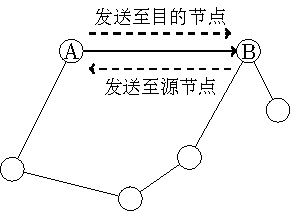
\includegraphics[width=0.4 \linewidth]{figures/triplet.pdf}\\
  \caption{Triplet操作示意图}{Triplet operations illustration}
  \label{fig:triplet}
\end{figure}

在计算城市人口流入量的时候,aggregateMessages接口中map操作选择将消息发送给有向边的目的节点;在计算城市
人口流出量的时候,map操作选择将消息发送给有向边的源节点,在reduce阶段所有消息汇总。
将上述两步生成的结果进行join和mapValue操作,计算每个城市的人口流动流出比,
算法流程见图\ref{fig:populationstatistic}。
\begin{figure}
  \centering
  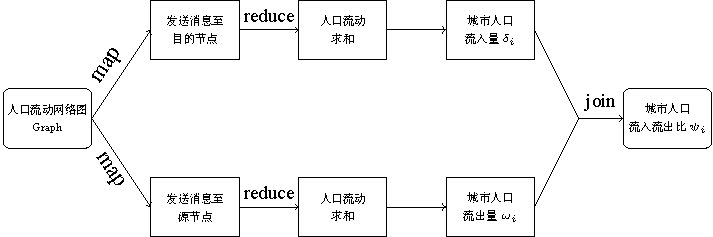
\includegraphics[width=0.9 \linewidth]{figures/population_statistic.pdf} \\
  \caption{人口流动统计流程图}{Flow chart of population statistic}
  \label{fig:populationstatistic}
\end{figure}

\subsection{统计分析}
以全国地级市和直辖市边界为空间查询范围,使用aggerateMessages函数分别计算出各自的流入量$\delta_i$、流出量$\omega_i$和流入
流出比$\psi_i$,结果栅格化渲染结果见图\ref{fig:flowinout}。
\begin{figure}
  \centering
  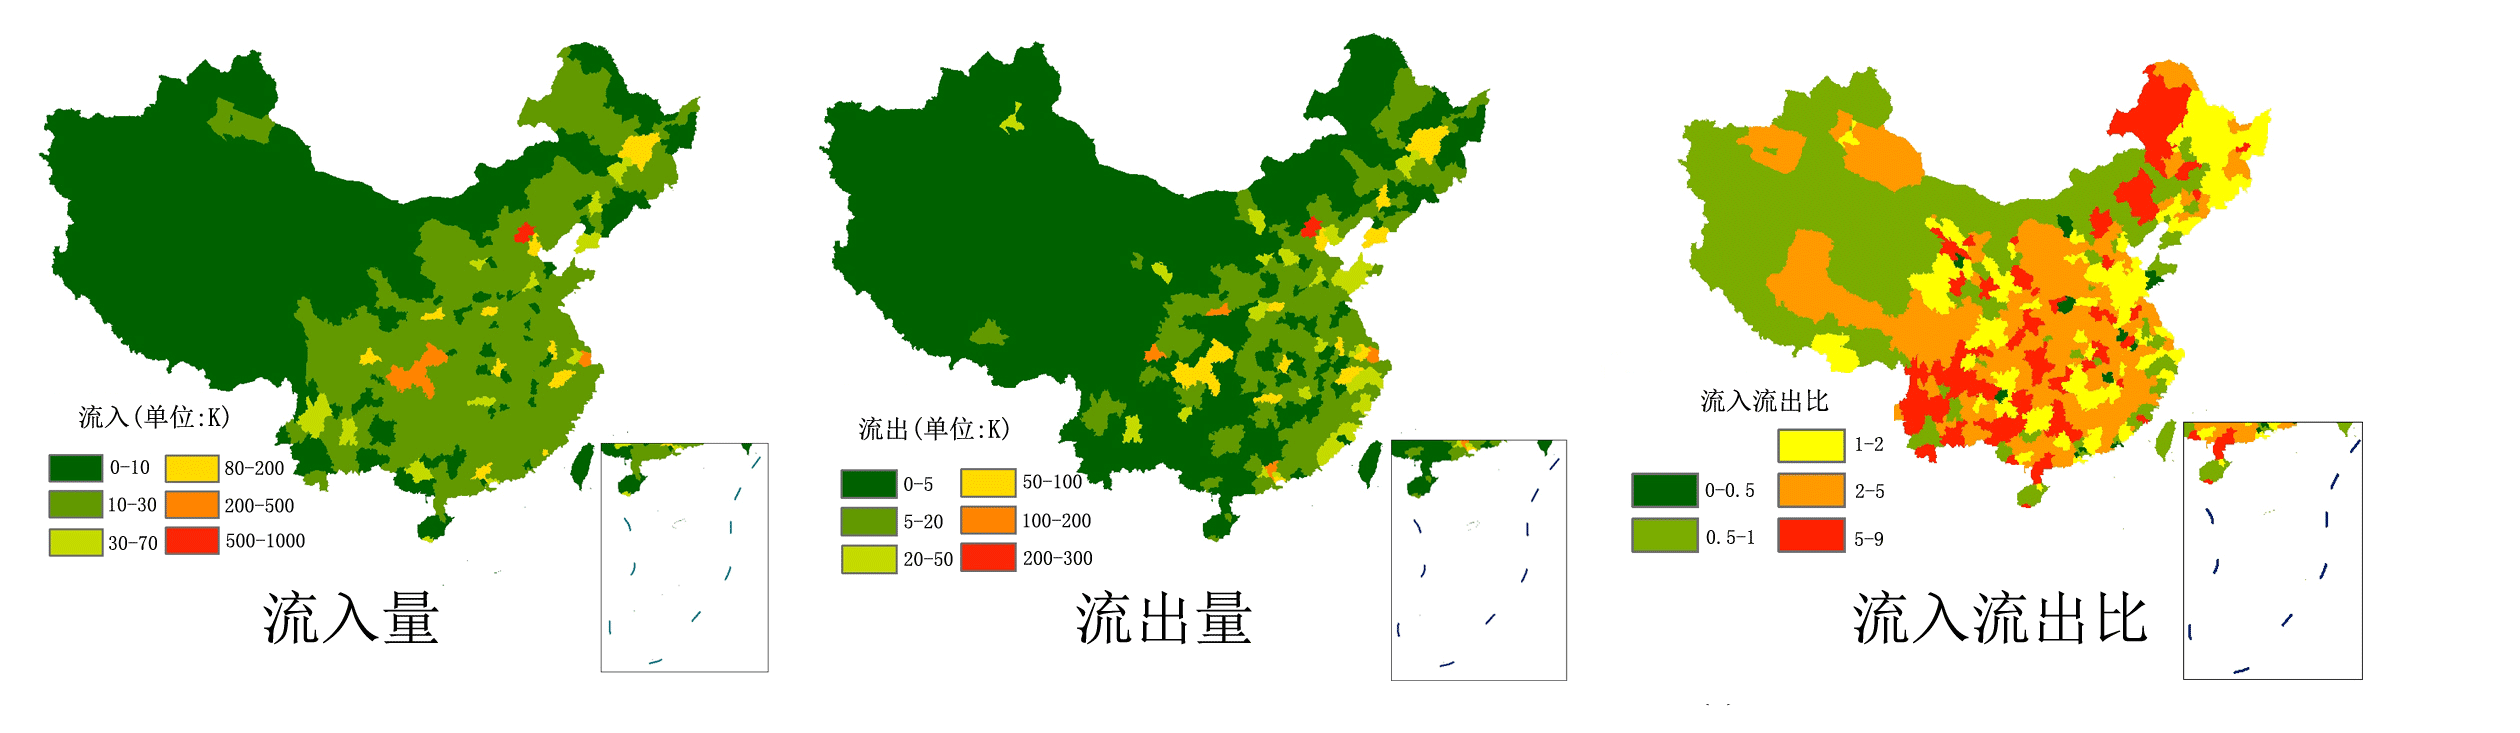
\includegraphics[width=13cm,height=4cm]{figures/flowratio.png} \\
  \caption{流出、流出和流入流出比}{Flow-in,flow-out and flow-ratio}
  \label{fig:flowinout}
\end{figure}

统计各个城市的人口流动数目,发现成都、西安、北京、广州、郑州等地为全国人口流动集中城市\cite{曹盼盼全国}。
并且人口流动量前$20\%$的城市占全国总用户的$70.1\%$,符合人口统计学和社会科学的「$80/20$法则」,
即$80\%$的事物或现象集中在前$20\%$的研究对象中。将前$20\%$城市人口流动统计见图\ref{fig:Populationstatistic},
可以看出人口流动流动量符合幂律分布(Power law)分布。
\begin{figure}
  \centering
  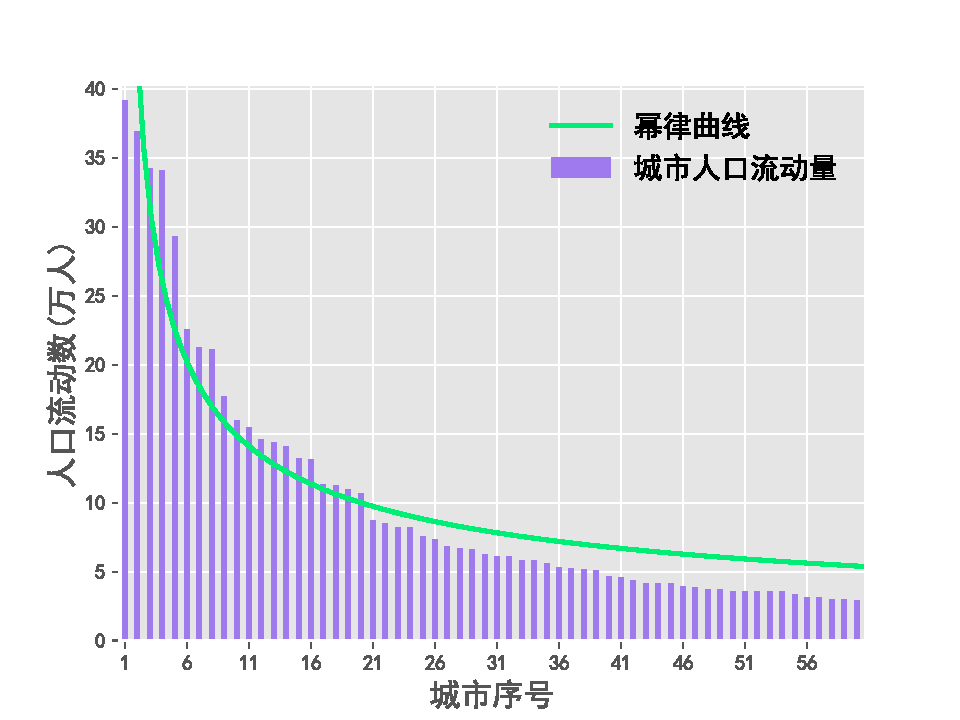
\includegraphics[scale=0.8]{figures/statisic.pdf} \\
  \caption{人口流动统计图}{Population flow statistic of cities}
  \label{fig:Populationstatistic}
\end{figure}

从图\ref{fig:flowinout}看出城市流入流出比呈现较多的复杂性:$\psi_i$远大于1表明该城市在春节期间人口呈现流入趋势;
$\psi_i$远小于$1$表明该城市在春节期间人口呈现流出趋势;而接近于$1$表明该城市人口在春节期间流动量持平,
主要城市的$\psi_i$见表\ref{tab:citiesinout}。
\begin{table}
  \centering
  \caption{城市流入流出比}{Cities' flow ratio}
  \label{tab:citiesinout}
  \tabulinesep=1.5mm
  \begin{tabu}to 1.0\linewidth{X[2,c,m]X[1,c,m]X[5,l,m]}
    \tabucline[0.1em]-
    \rowfont[c]{} 流入流出比$\psi_i$ & 说明 & 城市 \\
    \tabucline-
    大于1 & 流入 &   辽源、鄂州、西双版纳、毕节、永州、七台河、娄底、
                    姿阳、白色、黄冈、松原、三亚、娄底、大理等 \\
    接近1 & 持平 &  上海、北京、成都、武汉、哈尔滨、嘉兴、杭州、
                    长沙,广州、西安、太原、郑州、沈阳、乌鲁木齐等 \\
    小于1 & 流出 &  东莞、马鞍山、芜湖、青岛、苏州、深圳、包头、宁波、无锡、唐山,石家庄、呼和浩特等 \\
     \tabucline[0.1em]-
   \end{tabu}
\end{table}

流入流出比远大于$1$的城市主要有:\circled{1}春节返乡人群所在的城市,主要分布在人口劳动力输出的中西部城市,
四川、贵州、湖南、湖北等省份;剩余部分城市位于东北地区。\circled{2}南方著名旅游城市,海南,云南等省份。
随着旅游等第三产业发展,越来越多的人选择春节假期去度假,而不是回乡团聚,这些使得旅游城市在春节期
间迎来较大的人流量。

流入流出比接近$1$的城市春节期间人口流入量与流出量大致相同,这些城市主要是某个区域的连接中心,一般为省会城市,
如上海,北京,成都,武汉等等。

流入流出比小于$1$的城市主要有:\circled{1}沿海以劳动密集型产业发展起来的移民城市,集中在长三角和珠三角地区,据公安部最
新数据表明,深圳市常住人口超过$1300$万,但本地人口只有$250$万,外来人口超过$80\%$,位列全国第一,苏州以$50\%$外来人口排
名第二。\circled{2}重工业城市,其中以钢铁为代表重工业发展起来的城市如包头(包钢),唐山(首钢),马鞍山(马钢)等,人口
的流出可能与目前这些钢铁产业发达的城市产能过剩相关\cite{冯梅陈鹏钢铁}。

对人口流入流出比较大的城市,对这些城市交通、旅游等部门提供了决策依据,如航班的规划、旅游服务部门提前做好准备工作等等;也可以
通过从中人口的流入量,窥探城市经济走向和市场的活力。

\section{人口流向分析}{Analysis of Floating Population Route}

全国城市之间流动网络见图\ref{fig:citiesflow},从图中可以看出人口流向存在着不均衡性,明显的东部、中部和西部阶梯之分,
东部地区城市之间流动量大,流动密度强,中部地区次之而西部地区最小。
\begin{figure}
  \centering
  \includegraphics[scale=0.6]{figures/flow.jpg} \\
  \caption{城市人口流向}{Cities' population flow}
  \label{fig:citiesflow}
\end{figure}

\subsection{PageRank算法}
PageRank算法是Google搜索引擎的核心技术\cite{Boldi2009PageRank},该算法的核心思想
是将整个互联网抽象成网络图,每个网页抽象成一个节点,而节点之间的URL连接代表了网络图的边。
被许多重要页面引用的页面,往往还是重要的页面。算法开始假设所有节点拥有相同的权重,根据节点
的之间的链接权重设计出转移矩阵,通过权重转移矩阵相乘,重新分配权重,不停迭代循环,直至节点权重收敛。

以人口流动为例,将城市抽象成有向网络图中的各个节点,人口的流动抽象成节点之间的连通路径,构建出每个城市之间的流动矩阵$M$:

\[
  M=
\begin{bmatrix}
\alpha_{11} & \alpha_{12} & \ldots & \alpha_{1n} \\
\alpha_{21} & \alpha_{22} & \ldots & \alpha_{2n} \\
\ldots & \ldots & \ddots & \ldots \\
\alpha_{1n} & \alpha_{2n} & \ldots & \alpha_{nn} \\
\end{bmatrix}
\]

式中$\alpha_{ij}$为$i$城市人口流动至$j$城市的概率:
\begin{equation}
\label{eq:netprobability}
\alpha_{ij} = 
\left \{
  \begin{array}{cl}
  \frac{\beta_{ji}}{\sum_{k=0}^{k=n,k\ne i}\beta_{ki}} & i\ne j \\
  0 & i=j \\
  \end{array}
\right.
\end{equation}

式\eqref{eq:netprobability}中$\beta_{ki}$为在$k$城市微博用户中,账户位置为$i$城市的用户数量。
假设初始城市权重是相同的,即:
\begin{equation}
\label{eq:initalweight}
 V_0=
  \begin{bmatrix}
  1/n & 1/n & \ldots & 1/n 
  \end{bmatrix}^{T}
\end{equation}

通过$n$次迭代$V_n=M\times V_{n-1}$,直至$V_i$收敛,计算出每个城市在流动网络中的权重。

\subsection{城市流动网络权重}
GraphX模块中Graph类实现了PageRank算法,分为两种实现方式:一种是给定迭代次数的静态方法;另一种是给定
迭代收敛阈值的动态方法。本文选择动态方法,给定收敛阈值$0.0001$,计算得到权重前$20$位的城市见表\ref{tab:citiespagerank}。
\begin{table}
  \centering
  \caption{城市Pagerank排名}{Cities' Pagerank rank}
  \label{tab:citiespagerank}
  \tabulinesep=1.5mm
  \begin{tabu}to 1.0\linewidth{X[1,c]X[1,c]X[2,c]|X[1,c]X[1,c]X[2,c]}
    \tabucline[0.1em]-
    序号 & 城市 & PageRank值 & 序号 & 城市 & PageRank值 \\
    \tabucline-
    $1$ &   北京 & $0.058$ & $11$ & 厦门 & $0.014$  \\
    $2$ &   成都 & $0.033$ & $12$ & 哈尔滨 & $0.013$ \\
    $3$ &   上海 & $0.031$ & $13$ & 南京 & $0.012$ \\
    $4$	&   西安 & $0.028$ & $14$ & 长沙 & $0.012$ \\
    $5$ &   广州 & $0.026$ & $15$ & 沈阳 & $0.012$ \\
    $6$ & 	武汉 & $0.024$ & $16$ & 天津 & $0.011$ \\
    $7$ & 	杭州 & $0.017$ & $17$ & 长春 & $0.010$ \\
    $8$ & 	郑州 & $0.016$ & $18$ & 大连 & $0.009$ \\
    $9$ &	  深圳 & $0.015$ & $19$ & 济南 & $0.009$ \\
    $10$ &  重庆 & $0.014$ & $20$ & 太原 & $0.008$ \\
     \tabucline[0.1em]-
   \end{tabu}
\end{table}

以国家统计局2015年全国各直辖市、地级市和自治州的GDP数据,与城市人口流动网络权重进行相关性分析。
发现相关系数达$0.8$,表明呈现正相关关系,绘制散点图如图\ref{fig:rankgdpcorrelationanalysis}左
所示。为了更好的进行回归分析,将权重的平方根作为应变量,城市GDP数值作为响应变量,进行线性回归分析,结果如
图\ref{fig:rankgdpcorrelationanalysis}右所示,回归方程为:$\text{GDP} = 1.037\times 10^5 rank^{0.5}-2669$,
回归系数$\text{P-value} < 0.001$,通过假设检验。
\begin{figure}
  \centering
  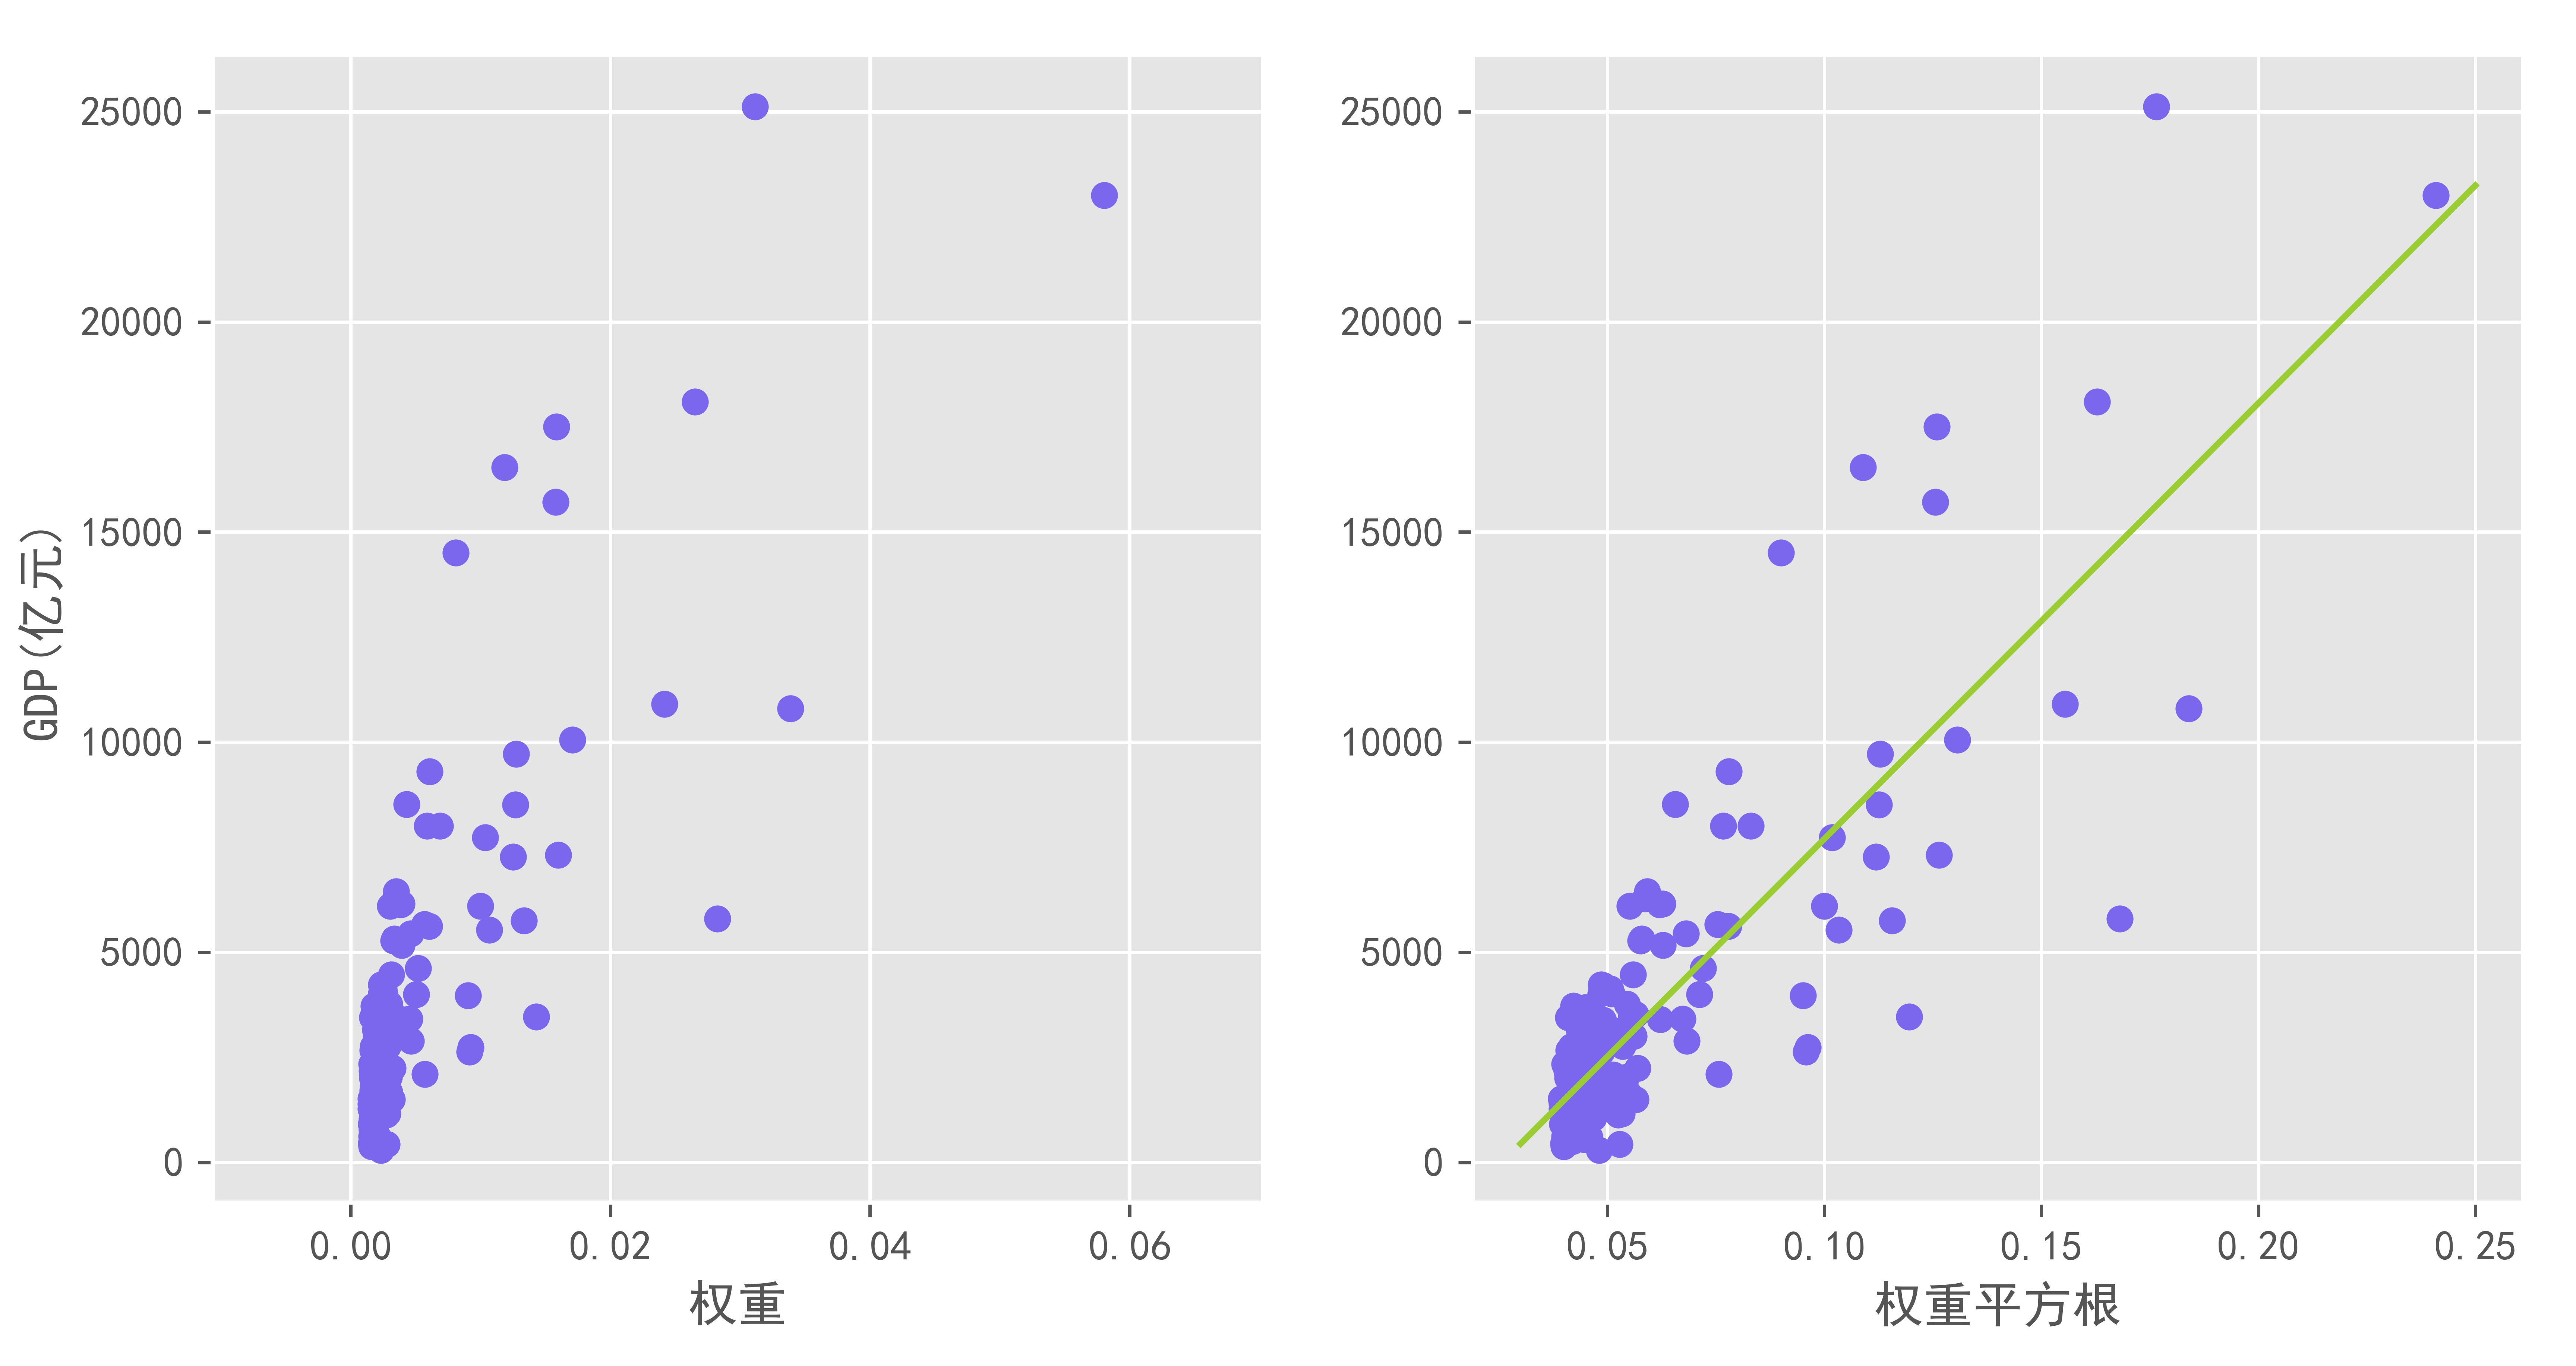
\includegraphics[scale=0.6]{figures/rank_gdp_scatter.png} \\
  \caption{权重和GDP相关性分析}{Ranks \& GDP correlation analysis}
  \label{fig:rankgdpcorrelationanalysis}
\end{figure}

从图\ref{fig:rankgdpcorrelationanalysis}中可以看出,并不是所有的点都很好的拟合回归曲线,存在「异常」
点。杠杆值可以描述点对整体回归的影响,高杠杆值可以说明改点属于异常点。据此绘制上述回归分析的残差平方与杠杆值散点图
,见图\ref{fig:residualLeverage},图中右下方和左上方的点属于异常点。
\begin{figure}
  \centering
  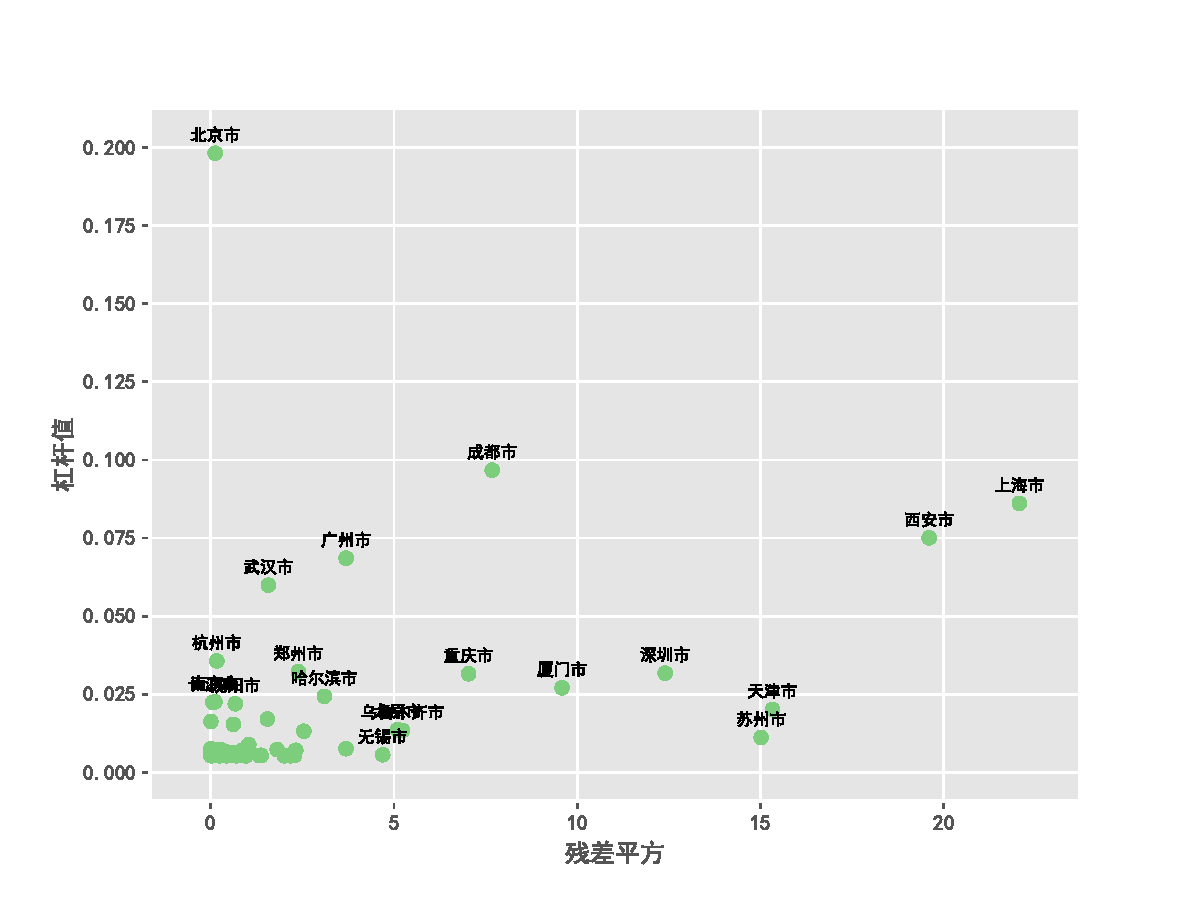
\includegraphics[scale=0.6]{figures/leverage.pdf} \\
  \caption{残差平方与杠杆值散点图}{Residual square \& leverage scatter plot}
  \label{fig:residualLeverage}
\end{figure}

城市特定时间段内在人口流动网络中的权重与实体城市权重存在明显的关系,出现了以下特征:

(1)城市权重与城市经济发展相对一致性。城市的权重与城市GDP呈现一定的正相关关系,
即城市的权重越高,城市的GDP数值会高。图\ref{fig:residualLeverage}中也表明了
在相关关系中异常点,主要分为两种:\circled{1}北京、成都、广州和武汉等城市权重
超出该城市GDP数值,其中北京最为明显;\circled{2}上海、西安、天津、苏州和深圳市等城市
的GDP发展远远大于该城市权重。

(2)城市权重在流动网络层级分布。通过对各个城市PageRank值分层,北京作为第一层级,是全国人口流动网络的中心;成都、上海、
西安、广州和武汉为第二个层级,是全国人口流动网络节点的副中心;杭州、郑州、深圳、重庆、厦门等为第三个层级,是区
域人口流动网络的中心;哈尔滨、南京、长沙、沈阳和天津等为第四个层级,是地区人口流动网络的中心。

(3)东部城市与中西部城市权重的差异明显。城市权重也符合「$80/20$法则」,排名前$20$城市权重和$0.81$。按照东部、中部、
西部三大地区划分,东部地区城市权重和$0.51$,中部地区城市权重和$0.32$,西部地区城市权重和$0.17$。虽然中部、西部地区也存在着权
重较高的城市,但东部区域在城市权重平均水平上明显高于中部和西部,因此东部城市在人口流动网络中扮演重要的角色。


\section{人口流动网络社群挖掘}{Community Mining of Floating Population Network}

现实世界中诸多系统都是以网络的形式存在,如人际关系网、机构协作网络、万维网等,这些统称为复杂网络(Complex Network),
可以通过简单的观测可以发现小规模网络的的特征、内部特征和划分,但是对于大规模和超大规模的网络,直观的显示很难通过肉眼发现
网络的特征和行为,因此需要使用复杂网络分析手段进行处理\cite{Girvan2002Community}。

网络社群挖掘(Community Mining,CM)是复杂网络聚类中研究最多的方法,社群挖掘方法对分析复杂网络中的拓扑结构,理解
复杂网络中隐藏的规律和预测复杂网络的行为不仅有重要的理论意义,而且有广泛的应用前景。城市之间人口流动也是属于一种复杂
网络,对该网络进行社群挖掘能够有效的发现城市在人口流动的联系,反映全国城市人口流动聚集效应。

\subsection{社群挖掘算法}

社群挖掘作为网络研究的经典问题,一直受到学者的广泛关注,目前社群挖掘算法主要有:GN(Girvan Newman)算法,定义边的介数,
依次删去介数最大的边,每次删除更新边的介数,如此循环,该算法在求解介数的时间复杂度较高\cite{Girvan2001Community};
LP(Label Propagation)算法使用邻居节点信息决定当前节点的社群,也可以应用到多社群挖掘,但是结果存在震荡问题,性能
不稳定\cite{Raghavan2007Near}。目前应用最多的是基于模块(Modularity)法,通过对比社群挖掘结果与随机图的差异判断社群划分的优劣,
研究表明基于模块值算法策略性能最好\cite{Newman2006Modularity}。

基于模块值算法通常先假设网络满足某种统计分布,进而通过极大似然估计方法得到网络社群。核心思想为模块值$Q$最大化,
见式\eqref{eq:qdefinition},$Q$是评价网络社群划分的优劣的质量指标。
\begin{equation}
\label{eq:qdefinition}
Q=\frac{1}{2m}\displaystyle{\sum_{vw}\big(W_{vw}-P_{vw}\delta(C_v,C_w)\big)}
\end{equation}

其中$W_{vw}$为网络中节点$v$和节点$w$之间的权重;$m$为权重之和;$P_{vw}$为零模型中节点之间的期望权重;$C_v$表示节点$v$所属的社群
的类别,如果节点$v$和节点$w$所属同一个社群,则$\delta(C_v,C_w)$为1,否则为0。

模块法开始将每个节点视为$N$个独立社群,选择使$Q$值增大最多或减少最小的连个顶点进行社群合并。
例如$A,B$连个社团合并,$a_i$为社团$A$中的成员,$b_j$为社团$B$中的成员,合并后的$Q$的
改变量用$\Delta Q$表示公式\eqref{eq:updateQ},$\Delta Q$为一个矩阵,其元素$e_{ij}$为社团$i$和
社团$j$合并后$Q$的变化值。%则社团合并后,因为合并无边相邻的社团对不能导致$Q$的增加,只需要考虑哪些相互之间有边的社团对。
\begin{equation}
\label{eq:updateQ}
\Delta Q_{AB}=Q_{AB}-Q_{A}-Q_{B}=\frac{1}{2m}\displaystyle{\sum_{a_i \in A, b_j \in B}}\bigg\{ \big( A_{ij} - \frac{k_ik_j}{2m} 
   \big) \times \delta \big[ r(i),r(j) \big] \bigg\}
\end{equation}

合并之后,对应的$\Delta Q$矩阵元素$e_{ij}$需要更新,如果选择让$A,B$社团合并为社团$D$,则新的社团$D$与其他社团之间(如社团$C$)
。在计算新一轮的合并$Q$时,易知$\Delta Q_{DC}=\Delta Q_{AC}+\Delta Q_{BC}$,上一次的迭代计算可以被
下一轮计算所采用,只需将$Q$矩阵中的$i,j$社团相关的行列相加,最多进行$n-1$次
计算来构建完整的社群划分\cite{Newman2012Communities}。

\subsection{社群挖掘算法并行化实现}

传统基于模块值社群挖掘算法是采用串行实现:逐个选择节点,选择合并社群,选择模块值最大的合并社群。而且需要两两考虑到
每个节点是否属于同一社群,算法时间复杂度将达到$O(n^2)$,当数据量急剧增加的时候,算法的时间消耗是可不接受的。因此
在并行计算框架下进行基于模块值进行社群挖掘,需要对公式\eqref{eq:qdefinition}简化为公式\eqref{eq:qdefinitionSimplify}。
其中$\sum_{in}$是社群$c$内部相互连接权重和,$\sum_{tot}$该社群$c$外部连接权重和。通过对比可以发现去掉了节点是否属于同一社群的判断
,避免了节点两两判断,简化了计算\cite{Blondel2008Fast}。
\begin{equation}
\label{eq:qdefinitionSimplify}
Q=\sum_{c}\big\{\frac{\sum_{in}}{2m} - (\frac{\sum_{tot}}{2m})^2\big\}
\end{equation}

判断某个节点$i$划分到其邻居节点计算模块值增益函数见公式\eqref{eq:updateQsimplify},其中$k_{i,in}$为节点$i$与社区$C$连接权重总和,
$k_i$为节点$i$与其余节点连接权重。
\begin{equation}
\label{eq:updateQsimplify}
\Delta Q=\big[ \frac{\sum_{in} + k_{i,in}}{2m} -(\frac{\sum_{tot}+k_i}{2m})^2 \big] 
      - \big[ \frac{\sum_{in}}{2m} - (\frac{\sum_{tot}}{2m})^2 - (\frac{k_i}{2m})^2 \big]
\end{equation}

算法主要分为两个步骤,第一步计算每个节点按照公式\eqref{eq:updateQsimplify}确定顶点$i$模块值增益最大进行合并社群,
第二步骤更新网络图,步骤见算法\ref{alg:communityMining}。
\begin{algorithm}[htbp]
\caption{社群挖掘算法}
\label{alg:communityMining}
\begin{algorithmic}[1]
\REQUIRE ~~\\
网络图:graph; \\
最多迭代次数: maxIterations;\\
模块值变化阈值: modularityThreshold;\\
\ENSURE ~~\\
模块值最大社群图: graph; \\
\STATE 初始化$C_i,\{i=1, 2,\ldots , N\}$
\STATE iterate=0
\WHILE{changeRate<modularityThreshold || iteration < maxIterations}
    \STATE changeRate=0
    \FORALL{$i$ in graph.vertexs} 
    \STATE $Q_i=[\quad ]$
    \FORALL{$j$ in $i$ neighbors}
    	\STATE $Q_i$ += $\Delta Q(i,j)$ $//$计算模块值增益
    \ENDFOR
    \STATE $Q_{max}$=max($Q_i$)
    \IF {$Q_{max} > 0$}
    	\STATE graph=updategraph() $//$如果最大模块值增益大于零,合并顶点
	\STATE changeRate= $Q_{max}$
    \ENDIF
    \ENDFOR
 \STATE iterate += 1 \\
\ENDWHILE
\RETURN graph
\end{algorithmic}
\end{algorithm}

算法\ref{alg:communityMining}每次迭代过程中依次选择图中的节点,对节点的所有的邻居节点尝试进行合并,对模块值增益最大且大于零的节点
进行合并。但是这种计算方式不利于并行计算框架,而且Spark RDD是不可变的数据结构,每次合并社群就要生成新的Graph对象,内存消耗非常大。
因此选择每次迭代更新多个节点,通过Graph类的aggregateMessages函数同时对图的所有边及其相关的节点进行同时操作,因此需要定义map阶段的
消息,按照公式\eqref{eq:updateQsimplify}的变量,定义如下消息结构。
\begin{lstlisting}[
  language=Java,
  morekeywords={implements, Integer, Long},
]
public class CombineMsg implements Serializable{
  public Integer degree;//该顶点的权重
  public Long commumity;//该顶点所属社区编号
  public Long commumityTotalDegree;//该社群权重总和
  public Long neighborDegree;//目标社群的权重
  public Long neighborCommumnity; //目标社群的编号
  public Long neighborCommumityTotalDegree;//目标节点的社群总权重
  public Long edgeWeight;//节点与与目标社群之间权重
}
\end{lstlisting}

对于发送到同一节点的消息集合,使用公式\eqref{eq:updateQsimplify},选择模块值增益值最大且大于$0$社群连边进行合并。
合并完毕后生成的消息图包含了本次社群合并连接顶点,并与原图进行joinVertice操作,完成图的更新。

由于所有边是并行操作,会出现「社群归属延迟」问题,如图\ref{fig:communityDelay}比如顶点$1$所在社群$c1$与顶点$2$所在社群$c2$进行合并,
而社群$c2$与顶点$3$所在社群$c3$进行合并,那么将会导致在joinVertice操作时候,这些顶点成为孤立的顶点。
从拓扑结构来看,社群$c1,c2,c3$应该属于同一个社群,因此对依据模块值增益生成的消息图计算连通分量,
直接使用Graph对象调用connectedComponents函数即可,最后与原图进行joinVertice操作,完成图的更新,流程示意图见图\ref{fig:Communitycombine}。
\begin{figure}
\centering
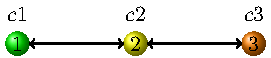
\includegraphics{figures/communitycombine.pdf}\\
  \caption{社群归属延迟}{Delay of commumity combine illustration}
  \label{fig:communityDelay}
\end{figure}

\begin{figure}
  \centering
  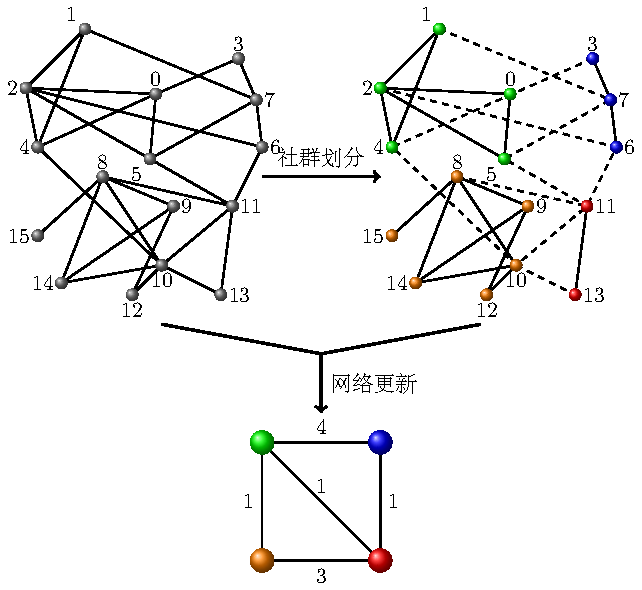
\includegraphics[scale=0.8]{figures/community.pdf}\\
  \caption{社群合并示意图}{Community combine illustration}
  \label{fig:Communitycombine}
\end{figure}

\subsection{城市社群挖掘}

由于人口流动往往存在较强的区域集聚性,在人口流动网络中体现出就是存在较强的社群结构,使用并行化
社群挖掘算法,反应全国城市人口流动的集聚效应\cite{杨小柳乡土中国}。对全国地级市和直辖市
人口流动网络进行社群挖掘,当整个人口流动网络划分为9个社群时,网络模块值最大,划分效果最好,
城市社群具体划分结果见图\ref{fig:nationalcommunitymining}和表\ref{tab:tbnationalcommunitymining}。
\begin{figure}
  \centering
  \includegraphics[width=10cm, height=8.115cm]{figures/commumity.jpg} \\
  \caption{全国城市社群划分}{National communities illustration}
  \label{fig:nationalcommunitymining}
\end{figure}
\begin{table}
  \centering
  \caption{全国城市社群划分详细}{National cities communities details}
  \label{tab:tbnationalcommunitymining}
  \tabulinesep=1.5mm
  \begin{tabu} to 1.0\linewidth{X[1,c,m]X[4,l,m]|X[1,c,m]X[4,l,m]}
    \tabucline[0.1em]-
    \rowfont[c]{} 社群&组成城市&社群&组成城市 \\
    \tabucline-
    1 & 北京、天津、河北城市、东三省城市、福建城市、三亚等 & 6 & 上海、江苏城市、安徽城市、浙江城市、丽江 \\
    2 & 山东城市 & 7 &广东城市、广西城市、湖南城市等\\
    3	& 河南城市	& 8	&重庆、四川城市、贵州城市等西南城市 \\
    4 & 山西城市 &	9 &	新疆城市、甘肃城市等西北城市 \\
    5	& 湖北城市、江西城市 & & \\
     \tabucline[0.1em]-
   \end{tabu}
\end{table}

对全国社群划分而言,也可以对其中的社群内部进一步使用社群挖掘算法,Spatial-Saprk强大的运算能力可以很容易的做到这一点,
比如上述全国社群1进一步使用社群挖掘算法,结果见图\ref{fig:subcommunity},每个社群中城市划见表\ref{tab:tabsubcommunity}。
\begin{figure}
  \centering
  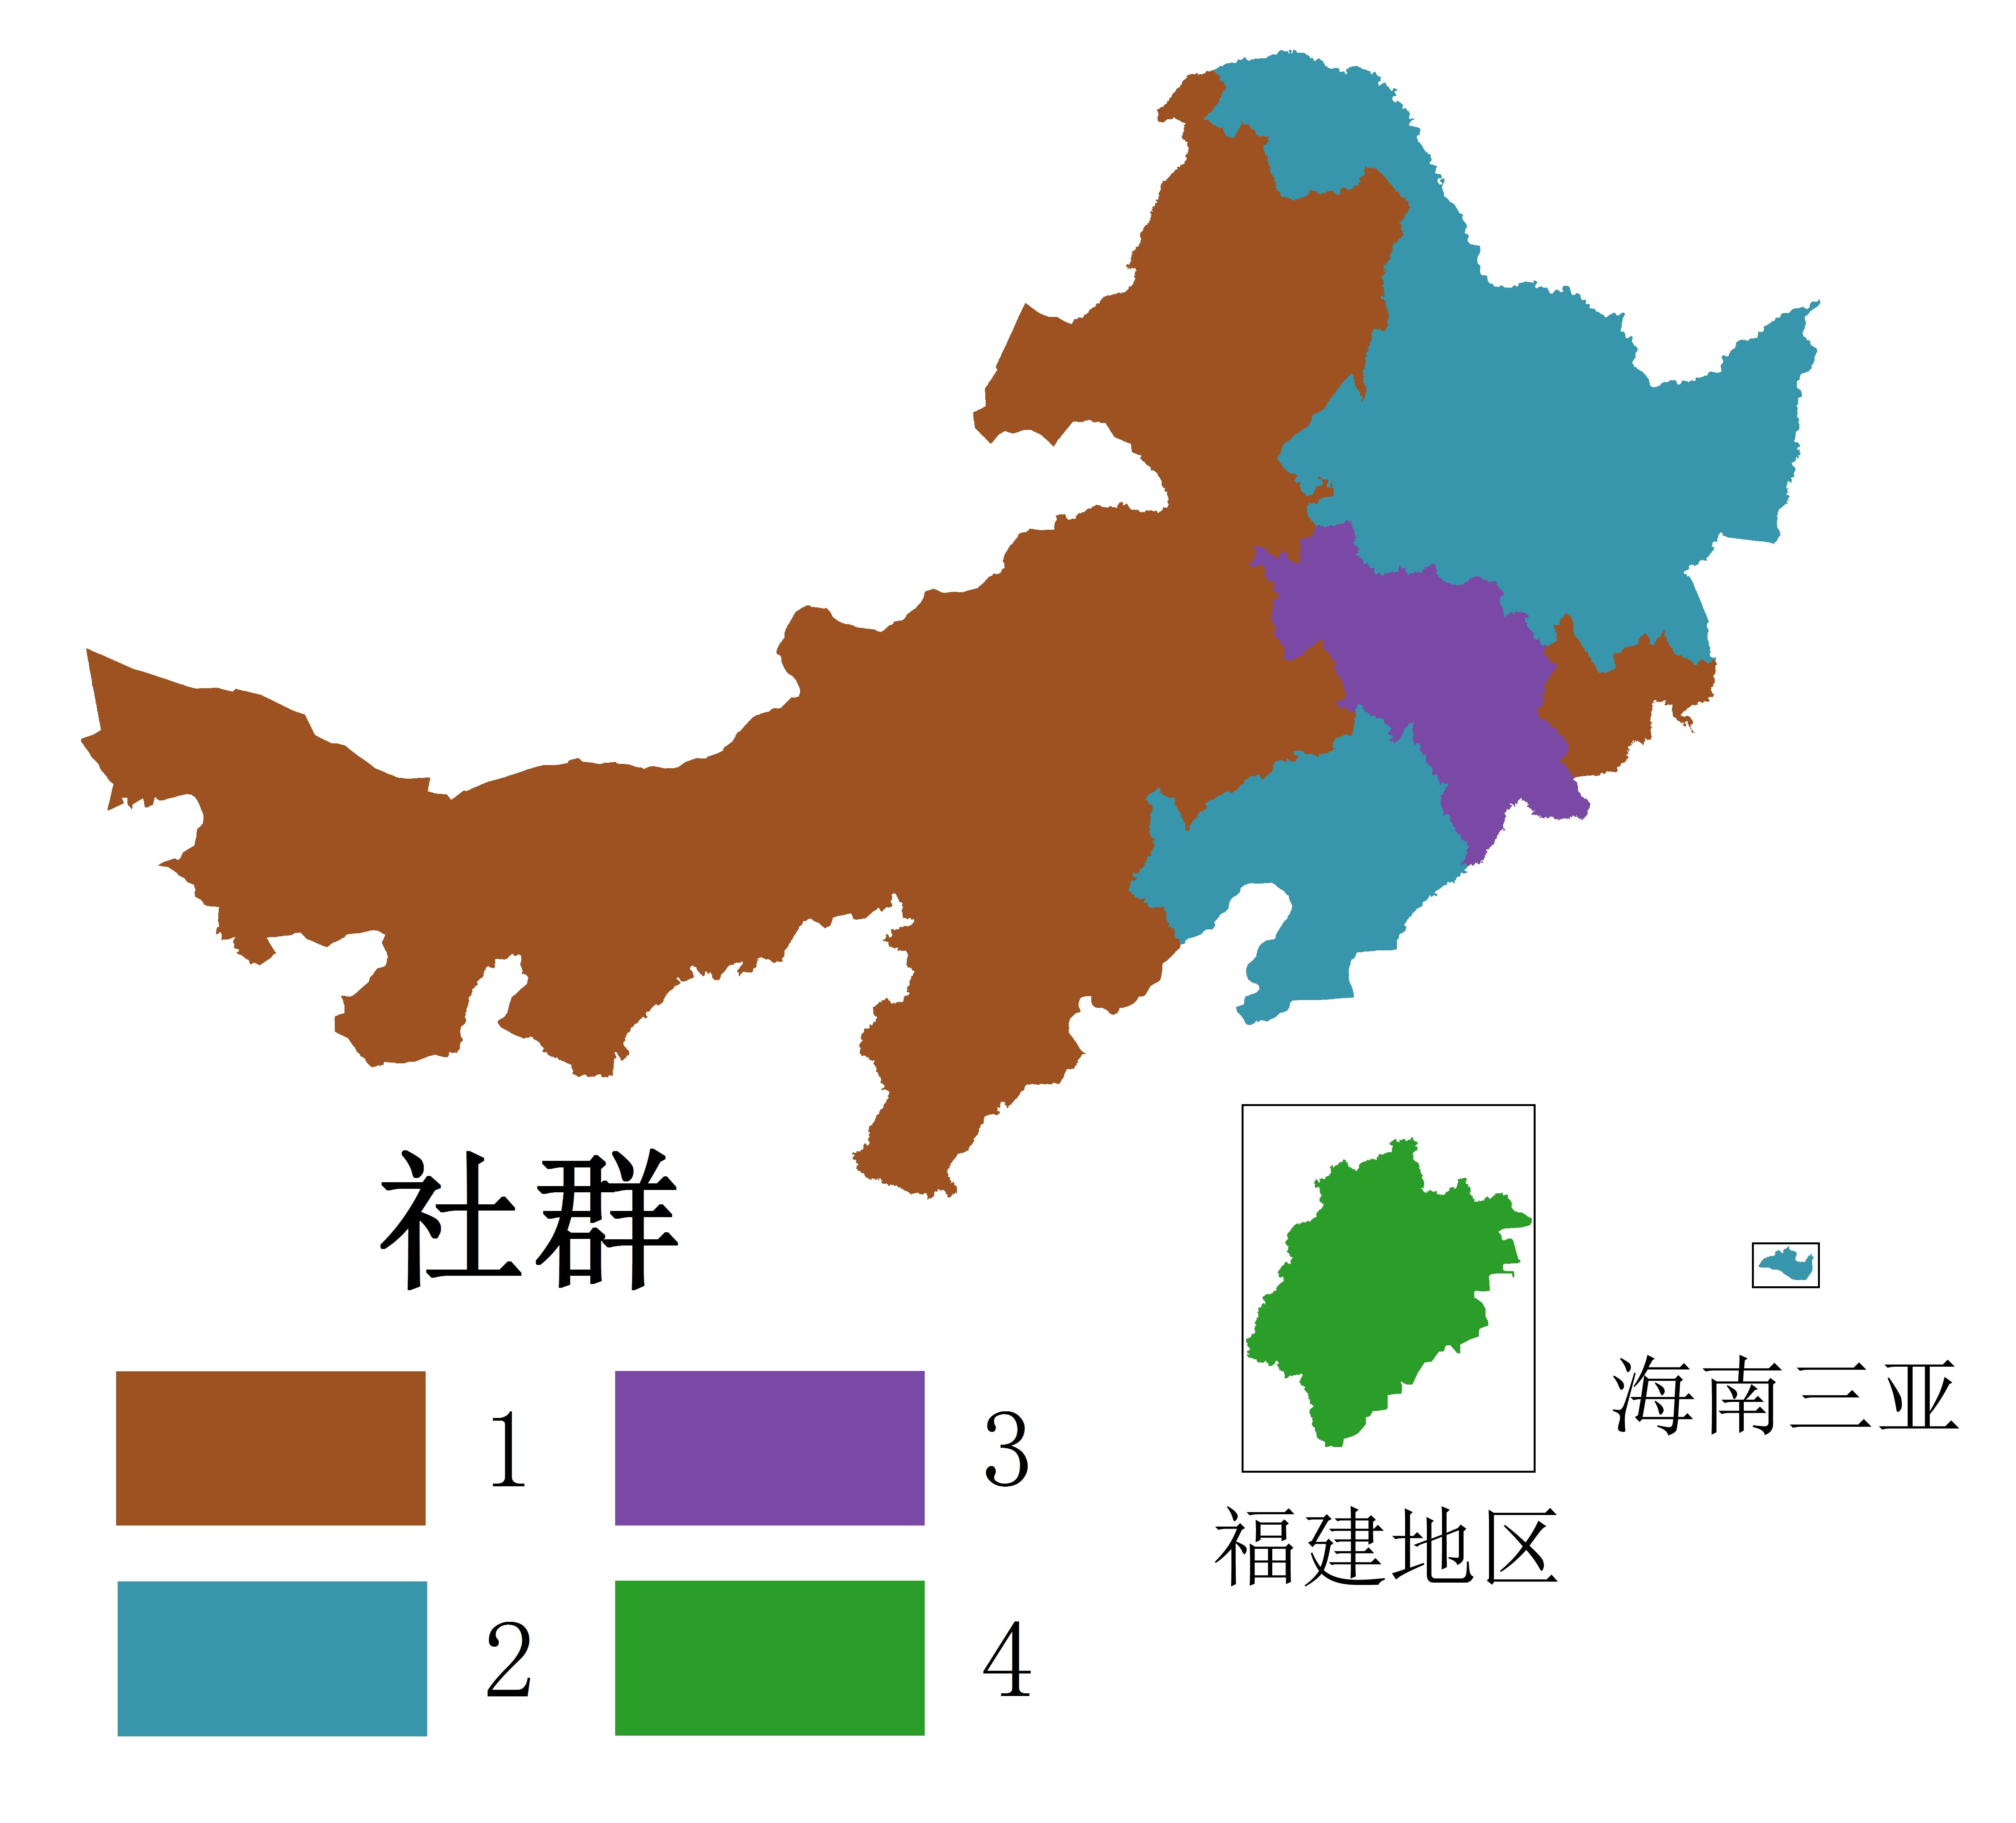
\includegraphics[width=8cm]{figures/subcommunity.jpg} \\ 
  \caption{子社群划分}{Sub-community illustration}
  \label{fig:subcommunity}
\end{figure}
\begin{table}
  \centering
  \caption{子社群划分}{Sub-community details}
  \label{tab:tabsubcommunity}
  \tabulinesep=1.5mm
  \begin{tabu} to 1.0\linewidth{X[1.2,c,m]X[6,l,m]|X[1.2,c,m]X[6,l,m]}
   \tabucline[0.1em]-
   \rowfont[c]{} 子社群 & 组成城市 & 子社群 & 组成城市 \\
    \tabucline-
   1 & 北京,天津,河北,内蒙古,吉林延边 & 2 & 黑龙江,辽宁,海南三亚 \\
   3 & 吉林城市 & 4 & 福建 \\
   \tabucline[0.1em]-
  \end{tabu}
\end{table}

分析每个社群的组成城市和城市之间地理空间分布,体现了以下特征:

(1)城市之间人口流动以省份为划分的特征较为明显,省份内部城市人口流动紧密
。以山东、山西、河南等省份为代表,其各自内部城市在人口流动网络中单独划分为一个社群。

(2)城市社群组成受地理空间位置影响较大,有明显的区域特征。在全国城市社群划分中,存在以北京为中心的
北方城市社群,上海为中心的东部城市社群,广东为中心的南部城市社群等集聚现象。

(3)城市社群组成也存在不受地理位置影响的特殊情况,如福建省的城市与北方城市组成同一社群,从侧面表
明其人口流动突破了地理空间的限制;丽江市与东部城市组成同一社群、三亚市与北方城市组成同一社群,
从一定程度表明这些旅游城市在春节假期的游客来源的组成。

(4)当对全国社群进行子社群进行社群挖掘,可以发现以省份为集聚现象越发明显,但是也可以发现少数城市与其他
省份人口联系更为密切,而这些往往是更值关注的内容,比如吉林的延边与北京、天津、河北等城市组成的社群更为
紧密,而海南三亚与黑龙江和辽宁组成的社群更为紧密。

通过对人口流动网络社群挖掘,可以快速地从海量数据中发现信息,这些信息既可以验证现实中已有的观念,如省份内部
人口流动紧密,空间邻近的省份人口交流频繁;也可以发现未知的现象,如福建省人口流动与北京、天津等省份城市
更为密切,海南三亚与北方城市尤其是黑龙江省份城市人口联系紧密。这些现象可以对省份和区域的决策者关于城市
规划、旅游航班调整、城市交通日常通勤等等方面提供很好的建议。

\section{本章小结}{Chapter Summary}

本章以全国新浪微博用户位置入手,构建了全国城市2016年全国城市人口流动网络,首先通过构建城市人口
流动指标,计算了城市人口流入、流出和流入流出比;借鉴PageRank计算每个城市在人口流动网络中的权重,
并与该城市GDP进行相关性分析,分析城市权重分布情况。最后对人口流动网络中进行社群挖掘,将全国城市
划分为9个社群,并分析了划分的特征。

\chapter{结论和展望}{Conclusion and Perspective}

\section{结论}{Conclusion}

为了高效处理海量空间数据,本文以Spark RDD为基础进行空间扩展,构建了
Spatial-Spark并行空间计算框架。以此框架为基础,对海量新浪微博空间数据进行有效
的分析,主要包括新浪微博POI数据和新浪微博用户位置数据分析和挖掘,并对
相关算法进行了并行化改进。

论文主要的工作及其成果总结如下:

(1)对Hadoop MapReduce和Spark并行计算框架进行分析,比较各自的优缺点。重点研究了
HDFS分布式存储策略和RDD的计算特点,分析Spark并行计算框架的优点,主要包括内存
计算带来的性能上优势和丰富的表现算子,为空间数据分析和挖掘提供了可能。

(2)以Spark为基础,对其进行空间方面的拓展,构建了并行空间计算框架Spatial-Spark,主要包括空间
数据分布式读写和空间数据变换,对基本的空间数据类型点、线和面分别拓展成为PointRDD、LineRDD
和PolygonRDD,并根据空间数据分布特征,提供了空间分区功能;
以R树为工具,对每个分区建立的空间索引,以加快空间数据分析速度。在此基础上,提供了
空间数据分析常用的模块,主要包含空间拓扑查询、KNN空间邻近查询和空间连接查询。最后搭建了分布式
Hadoop/Spark计算集群,验证了Spatial-Spark在空间数据处理方面的优势。

(3)分析了新浪微博提供的API接口,使用C\# SDK编写了获取新浪微博POI和全国新浪微博用户位置数据的
应用程序。

(4)研究了空间关联规则算法,重点分析了空间同位规则挖掘挖掘算,并结合Spatial-Spark提出了并行化
空间连接算法优化方案,对全国城市微博POI类别进行空位模式挖掘。首先针对上海、武汉和重庆三市进行
二阶模式挖掘,分析(高等院校、培训机构)模式在不同距离阈值下三市的空间参与度。选择空间距离阈值$d=500\text{\rm{m}}$和空间
参与度阈值$0.6$,对北京市进行同位模式挖掘,发现同位模式阶数越高,空间模式的数量越少,直至六阶,
(KTV,中餐厅,咖啡厅,甜品店,美容美发店,酒吧)为六阶空间模式的实例。由于新浪微博POI人为因素影响
较大,因此这些POI类别集聚的现象更加表达了现实线下人们活动现象,这对商家商业推广提供了很好的建议。

(5)新浪微博用户使用微博位置和用户账号位置形成人口流动,使用Spatial-Spark空间查询构建全国城市
在2016年春节期间人口流动网络图。首先根据GraphX并行计算功能,统计了各个城市人口流入量、流出量和流出
流出比,发现了全国城市人口流动情况的多样性;然后使用PageRank算法,计算出每全国城市在人口流动网络中
的权重并与城市GDP进行关联分析,发现城市权重与城市GDP发展相关联,并确定了各个等级区域人口流动网络的中心;
最后对整个人口网络进行进行社群挖掘,通过改进后模块值法,发现了全国城市人口流动社群,发现城市联系紧密性与省份有关,
地理位置对其影响很大,但也存在突破地理空间位置限制的城市。

\section{展望}{Perspective}

本文以新浪微博为研究内容,使用Spark进行了空间数据分析和挖掘进行了尝试,但是仍需在以下几个方面进行深入研究:

(1)空间连接分区索引使用:空间索引能有效地加快空间查询速度,但在Spatial-Spark上层空间连接模块中尚未有效
地使用已经建立的空间索引的进行加速算法,由于R树构造的特殊性,所以不能通过最小外包矩形进行Join操作。

(2)同位模式算法改进:在新浪微博POI类别同位模式挖掘中,使用全连接算法,虽然通过并行化改进在二阶模式
生成中减低了时间复杂度,但是在生成更高阶的过程中,RDD提供的join操作包含了较多的不满足条件的组合模式,因此
如果改进RDD在join操作的选择是值得研究的方向。

(3)微博数据获取方式改进:由于新浪微博API的限制性,不能获取关于用户的所有微博信息,因此在只能获取用户的
位置同时不能获取用户的历史微博数据,这些导致通过用户微博位置的注册地判断人口流动存在有偏性。如果采用网
络爬虫的方式,突破新浪微博API的限制,获取更多的用户的信息,那么将会发现更加有价值的信息。

\backmatter

%\bibliographystyle{cumt-num}
\bibliographystyle{new-cumt-num}
\bibliography{RefExam}

\begin{resume}

\section*{一、基本情况}


姓名: \zuozhe\quad 性别: 男\quad 民族: 汉\quad 出生年月: 1992-02\quad 籍贯: 江苏扬州

2010-09 --- 2014-07\quad  中国矿业大学环境与测绘学院工学学士;

2014-09 --- 2017-06\quad  中国矿业大学环境与测绘学院工学硕士.

\section*{二、学术成果}

\begin{enumerate}
  \item \zuozhe,土地确权内业处理软件,软件著作权,登记号:2015SR091014
\end{enumerate}


\section*{三、获奖情况}
\begin{enumerate}
  \item 2014-2015年度\quad 一等奖学金
  \item 2015-2016年度\quad 二等奖学金
  \item 2016-2017年度\quad 三等奖学金
\end{enumerate}
\section*{四、研究项目}
\begin{enumerate}
  \item 国家高分重点项目:中科院电子所苏州研究院, 2016, 参与;
  \item 国家自然基金项目:数字摄影测量目标精密定位于精度估计研究,编号:41171343, 参与;
  \item 山东省梁山县农村土地确权登记颁证项目,2014, 主要参与;
\end{enumerate}

\end{resume}

\GuanJianCi{Spatial-Spark, 新浪微博, 同位模式, 网络分析}
\BingLieTiMing{Analysis and Application about Internet Spatial Data Based on Spatial-Spark}
\LunWenYuZhong{中文}
\XueHao{TS14160005}
\PeiYangDanWeiDaiMa{10290}
\PeiYangDanWeiDiZhi{江苏省徐州市}
\XueZhi{三年}
\LunWenTiJiaoRiQi{2017 年 6 月}
\DaBianWeiYuanHuiChengYuan{王永波,杨化超,陈国良,刘志平}
\LunWenZiZhu{无}
%\XueWeiShouYuDanWeiMingCheng{}
%\XueWeiShouYuDanWeiDaiMa{}
%\XueWeiJiBie{}
%\LunWenTiMing{}
%\PeiYangDanWeiMingCheng{}
%\YouBian{}
%\XueWeiShouYuNian{}

\makebackcover
%\printindex
\clearpage
\end{document}
